\documentclass[a4paper,12pt]{article}
% \usepackage{floatrow}
% from documentation: "The floatrow package borrows core code from the float1 and rotfloat2 packages, so you must not load these packages.
\usepackage[subpreambles=true]{standalone}
% \usepackage{pdfpages}
\usepackage{ragged2e}
\usepackage{graphicx}
\usepackage{titlesec}
% \usepackage[T1]{fontenc}
\usepackage[OT1]{fontenc}
\usepackage{hyperref}
\usepackage{emptypage}
% \usepackage{fontspec}
\usepackage{wrapfig}
% \usepackage[export]{adjustbox}
% \usepackage[utf8]{inputenc}
\usepackage{subcaption}
%\usepackage[showframe]{geometry}
\usepackage{geometry}
\usepackage{tabularx}
\usepackage{titlesec}
\usepackage{geometry}
\usepackage{marvosym}
\usepackage{verbatim}
\usepackage{enumitem}
%\usepackage[hidelinks]{hyperref}
\usepackage{hyperref}
%\usepackage{fancyhdr}
\usepackage{fontawesome5}
\usepackage{multicol}
\usepackage{graphicx}
% \usepackage{cfr-lm}      % pdfLaTeX-only font pkg — conflicts with fontspec under XeLaTeX
% \usepackage[T1]{fontenc} % not needed with fontspec/XeLaTeX
% XeTeX-specific packages
\usepackage{fontspec}
\usepackage{amsmath}
% \usepackage{subfiles}
% \usepackage{minidocument}
\setlength{\multicolsep}{0pt} 
% \pagestyle{fancy}
% \fancyhf{} % clear all header and footer fields
% \fancyfoot{}
% \renewcommand{\headrulewidth}{0pt}
% \renewcommand{\footrulewidth}{0pt}
%https://www.freelance.pizza/post/build-a-stunning-engineering-portfolio
%https://www.reddit.com/r/AskEngineers/comments/fh4ql3/how_to_create_an_engineering_portfolio
% https://silo.tips/download/christopher-rhoades-engineering-portfolio
\geometry{left=0.5 in, top=0.5 in, right=0.5 in, bottom=0.5 in}
%\usepackage{tcolorbox}
%https://osl.ugr.es/CTAN/macros/latex/contrib/tcolorbox/tcolorbox.pdf, https://tex.stackexchange.com/questions/511802/how-to-draw-a-box-around-some-text
% \tcbuselibrary{breakable}
% \tcbset{
%   width=0.7\textwidth,
%   halign=justify,
%   center,
%   breakable,
%   colback=white    
% }
%\usepackage{framed}
\usepackage[most]{tcolorbox}
\tcbset{
	frame code={}
	center title,
	left=0pt,
	right=0pt,
	top=0pt,
	bottom=0pt,
	colback=gray!20,
	colframe=white,
	width=\dimexpr\textwidth\relax,
	enlarge left by=-2mm,
	boxsep=4pt,
	arc=0pt,outer arc=0pt,
 }
\usepackage[backend=biber,
    style=chem-acs, sorting = none]{biblatex}
\usepackage{sidecap}
\addbibresource{portfolio.bib}
\hypersetup{colorlinks=true, urlcolor=cyan, linkcolor=blue  }
\geometry{margin=0.5in}
%% This is the file `kultem.sty',
%% a non-official KU Leuven template.
%%
%% Copyright (C) 2021 by Henri De Plaen, KU Leuven.
%%
%% This file may be distributed and/or modified under the conditions of
%% the LaTeX Project Public License, either version 1.2 of this license
%% or (at your option) any later version.  The latest version of this
%% license is in:
%% 
%%    http://www.latex-project.org/lppl.txt
%% 
%% and version 1.2 or later is part of all distributions of LaTeX version
%% 1999/12/01 or later.
%%
%% I do not own the rights on the KU Leuven logo, which is by consequence
%% not covered by the license above.
\usepackage{fancyhdr}
% \renewcommand\maketitle{1}{\vfill\begin{center}\vspace*{3cm}{\textbf{\Huge\color{black}\@title}} \\[0.7cm]\ifdefempty{\@subtitle}{}{\textbf{\LARGE\color{gray}\{#1}}}\end{center}\begin{center}\vspace*{1cm}\textbf{\@author\\}\vspace*{1cm}\end{center}}
% \newcommand{\mytitle}[2]{
% \begin{flushleft}\vspace*{3cm}{\textbf{{#1}}} \\[0.7cm]{\textbf{\href{mailto:#2}{{#2}}}}\end{flushleft}}
\title{Jesse Shen Engineering portfolio}
%\author{}
\date{\today}
%@date\end{center}
\newcommand{\emaila}{Jesse12shen@gmail.com}
\setlength\parindent{0.05\textwidth}
\begin{document}
% \setmainfont{Arial}
% \frontmatter
%\maketitle{j.shen@wustl.edu}
% \mytitle{Jesse Shen}{j.shen@wustl.edu}

\newcommand{\mytitle}[2]{
%\begin{flushright}\vspace*{3cm}{\textbf{\LARGE{#1}}} \\[0.7cm]{\textbf{\LARGE Engineering Portfolio for Volta Labs Entry-level Fluidics R\&D Engineer}}\\[0.7cm]{\textbf{\LARGE\href{mailto:#2}{{#2}}}}\end{flushright}}
\begin{flushright}\vspace*{3cm}{\textbf{\LARGE{#1}}} \\[0.7cm]{\textbf{\LARGE Engineering portfolio}}\\[0.7cm]{\textbf{\LARGE\href{mailto:#2}{{#2}}}}\end{flushright}}
\begin{titlepage}
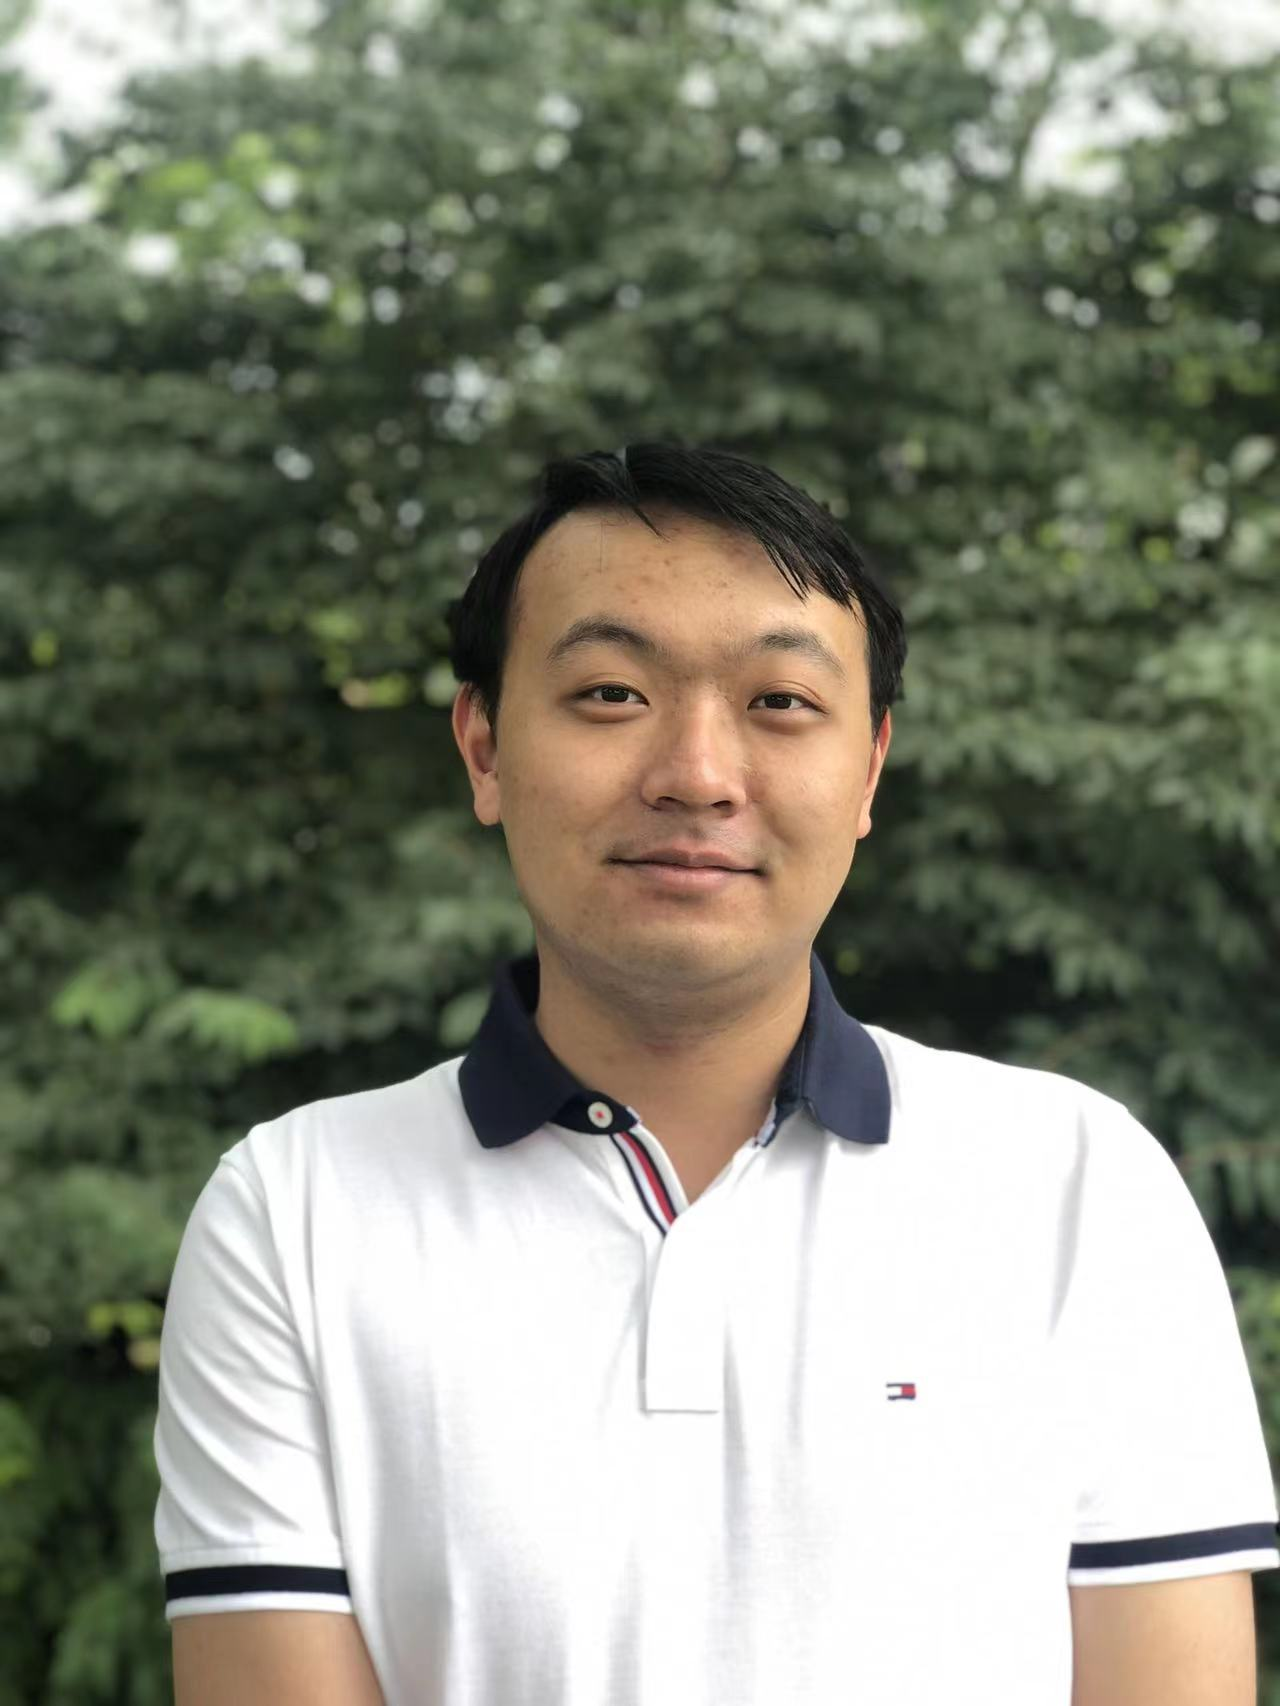
\includegraphics[width=5cm]{images/mmexport1655739259374 headshot.jpg}
\mytitle{Jesse Shen}{\emaila}
\end{titlepage}

\tableofcontents
%\mainmatter
\section{Introduction}
Hello! My name is Jesse and I am interested in this role because I want to apply my combination of experience with clinical research and AI solutions. 

Here in this portfolio you will find a few past research projects and my contribution to them in reverse-chronological order. Starting with my most recent research at Carnegie-Mellon's (CMU) Biomedical Engineering department, this portfolio will then go over some relevant class projects I did at CMU. I will also go into some more detail about my key contributions during my employment at the University of Minnesota followed with a section on work I did during my undergraduate studies at Washington University in St. Louis.
\section{Graduate research at Carnegie Mellon University's Department of Biomedical Engineering}
% \subsection{Introduction}
My research advisor at Carnegie Mellon University (CMU) was Siyang Zheng-- his research specialized in microfluidic devices and their applications. I had split my time between two projects and learned cell culture between these two projects. While I was initially admitted as a PhD student, funding issues and restructuring led to me mastering out.

My research at CMU gave me hands-on experience with biochemistry techniques and familiarized me with microfluidics and sequencing. The thymus-on-a-chip project taught me what goes into organ-on-a-chip research as well as giving me an opportunity to be deeply involved with immunoengineering. Meanwhile, preparing for methylation sequencing as part of the methylation-based cancer diagnostics project helped me understand how next-generation sequencing and AI could be applied in diagnostics.

\subsection{Thymus-on-a-chip}
\begin{wrapfigure}{r} {0.4\textheight}
% \vspace{-3cm}
%\vspace{-1cm}
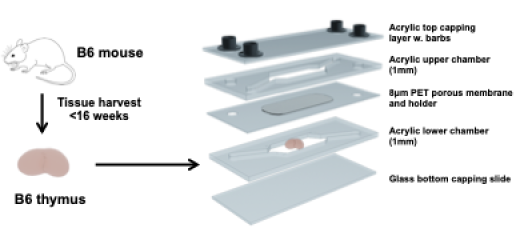
\includegraphics[clip, scale = 0.7]{images/TOC Figures 05_2020.pptx.png}
\vspace{1cm}
\caption{Acrylic version of thymus-on-a-chip diagram (\textit{Fan group unpublished manuscript})}
\label{fig: thymus chip}
% \vspace{-1cm}
\end{wrapfigure}
My primary project was the development of a thymus-on-a-chip. This project was a collaboration between my advisor and Yong Fan's immunology research group which had developed an improved thymus model in mice \cite{Fan}. While Dr. Fan's group had an initial acrylic design for a thymus-on-a-chip, I wanted to design a disposable PDMS version that would prevent contamination issues. A brief involvement with an acrylic version (Figure \ref{fig: thymus chip}) and laser cutting the compartments was where I was introduced to laser cutting and power tools. 

On the cell side, one protocol\cite{Campinoti} I sought to replicate was the characterization of expanded thymic epithelial cells. These researchers had developed a way to culture medullary thymic epithelial cells. During this time,  I also applied for fellowships outlining the potential for a thymus-on-a-chip to function as a T-cell factory -- with potential applications in T-regulatory cells to enable universal transplantation.

Up until the end of the project, I sought ways to control the risk of contamination. This issue proved to be a challenge during data collection and would end a week-long run of the organ-on-a-chip. However, my next steps were to adapt protocols in the literature that showed runs lasting for weeks \cite{Seet}.
% \vspace{-1cm}
\subsection{Methylation-based Cancer Diagnostics}
%bisulfite chemical reaction here?
My secondary project involved implementing improved cancer diagnostics. A research area of the Zheng laboratory is extracellular vesicle (EV) applications, in my case looking at genomic DNA in EVs for cancer diagnosis \cite{Liang}.

Epigenetics is an active area for cancer diagnosis, with methylated genes being identified as a biomarker for cancer. While researching potential diagnostic kits for methylation detection, I had gathered control data for singular genes (methylation-specific PCR) with plans to eventually scale up to multiple gene detection via next-generation sequencing.  

% \begin{wrapfigure}{l}{0.6\textwidth}
\begin{SCfigure}[1.0][h]
\vspace{-1cm}
    
    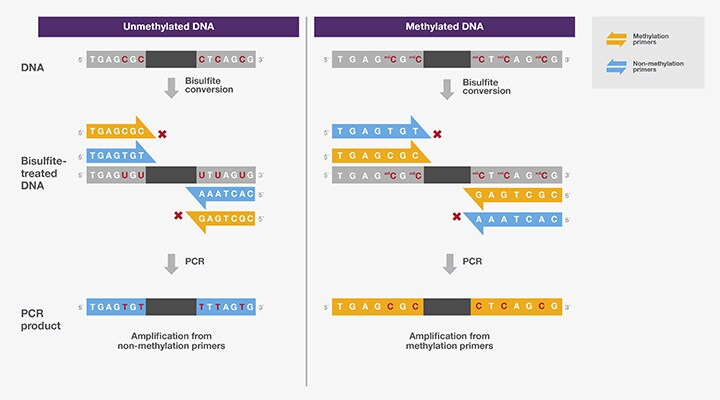
\includegraphics[clip, scale = 1.8]{images/1467318483869.jpg}
    \vspace{-0.5cm}
    \caption{Methylation-specific PCR diagram from Thermofisher website (\href{https://www.thermofisher.com/us/en/home/life-science/cloning/cloning-learning-center/invitrogen-school-of-molecular-biology/pcr-education/pcr-reagents-enzymes/pcr-applications.html}{thermofisher.com})}
\label{fig:1}
\end{SCfigure}
% \end{wrapfigure}
\newpage
\hspace{1cm}
\section{Graduate class projects at Carnegie Mellon University}
\subsection{\textit{Introduction to Deep Learning: 11-785}}

This class taught both the theory and practical applications of deep neural networks. One of the requirements included a group project which my team decided on a cancer prediction model based on patient electronic medical record data (Figure \ref{fig: placido1}). My role was implementing the baseline transformer model and going through an  expansive Github repository from the paper that inspired our project \cite{placido2023}. Other elements of the class included training and implementing methods/functions from: 1.) multilayer perceptrons for speech recognition 2.) convolutional neural networks for facial classification 3.) long short-term memory with uneven lengths of sequences for speech recognition 4.) transformers for speech-to-text functionality. All models were implemented in Pytorch, using large datasets with homework assignments having Kaggle test competitions.
\begin{figure}[h]
\begin{center}
% https://www.baeldung.com/cs/latex-subfigures so the problem is caption sharing?
\subfloat[Figure
snippet from reference \cite{placido2023}. Describing the learning and prediction portions of the machine learning workflow. \textbf{Learning:} how the input data is set up and fed into the machine learning model followed by the model's output. \textbf{Prediction:} the pipeline for the model's inference and the practical impact.]{
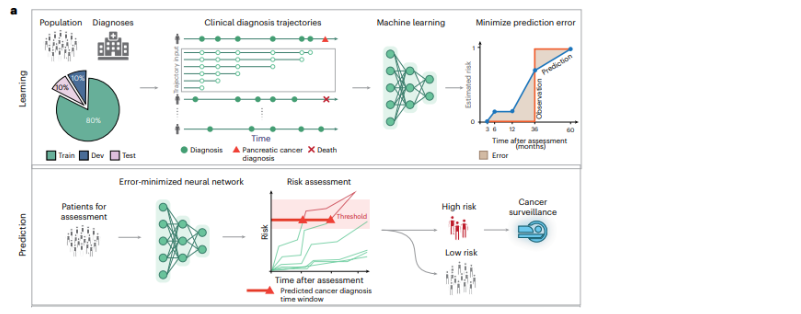
\includegraphics[trim={0 0 3cm 0}, clip, scale = 1.2]{images/placido fig1a.png}
% \vspace{-5.5cm}
\label{fig: placido_a}
%\vspace{1.0cm}
}
\caption{Visualization of the pipeline of input data (patient medical records) to risk assessment and its outputs and impact. Figure from reference \cite{placido2023}}
\label{fig: placido1}
\end{center}



% 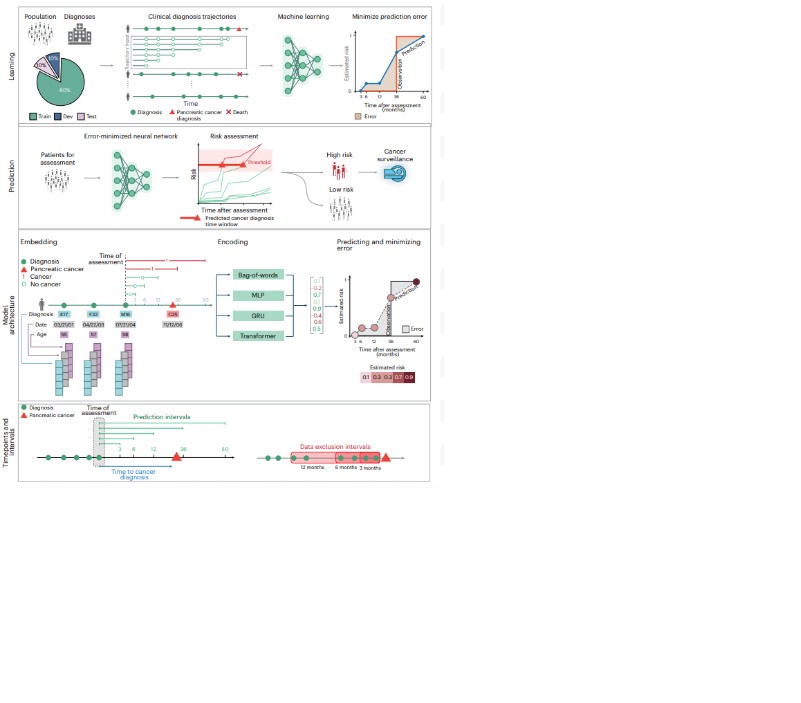
\includegraphics[trim={0 0 5cm 0},clip,scale=1.1]{images/Placido fig1.png}
% \caption{Figure
% snippet from reference \cite{placido2023} describing the pipeline of input data (patient medical records) to risk assessment and its practical procedure.  and functions of the }
% \label{fig: placido1}
\end{figure}
\newpage
\begin{figure}[h]
\ContinuedFloat
\begin{center}
\subfloat[Figure
snippet from reference \cite{placido2023}. Details on the model's process: embedding of patient visits, encoding based on various deep learning architectures, the specific prediction of interest based on time of assessment.]
{
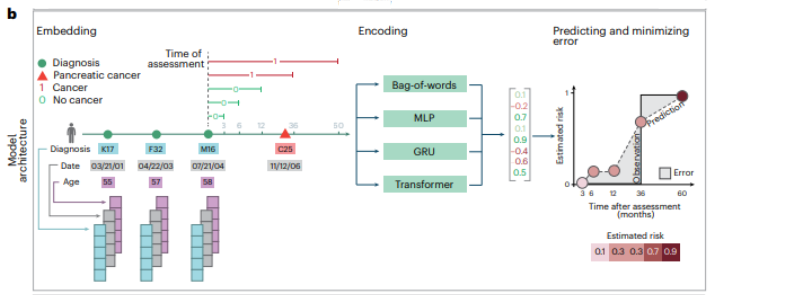
\includegraphics{images/placido fig1b.png}
\label{fig: placido_b}
}
\end{center}
\begin{center}
\subfloat[Figure
snippet from reference \cite{placido2023}. Details on how time of assessment is assigned.]
{
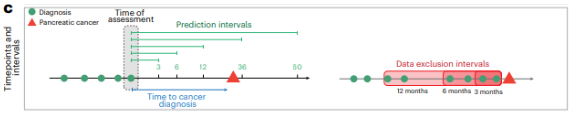
\includegraphics[scale=1.3]{images/placido fig1c.png}
\label{fig: placido_c}
}
\end{center}
\caption{Visualization of the pipeline of input data (patient medical records) to risk assessment and its outputs and physician response. Figure from reference \cite{placido2023}}
\end{figure}
% \subsection{\textit{Introduction to Machine Learning: 10-601}}
% This class was where I picked up python-- specifically numpy and matplotlib because other python packages were restricted. I learned about the many different algorithms that were used and the requirements for each type of model.
% as well as the current predominance of neural networks in the field. One assignment was a One Hidden Layer Neural Network depicted in Figure \ref{fig: NN} done with module/class-based automatic differentiation. The task was supervised image classification of 10 letters in the OCR dataset.

%\begin{wrapfigure}{r} {0.7\linewidth}
% \begin{figure}[h]
% %\hspace{-2cm}
% % \vspace{-0.7cm}
% %\fbox{
% %\hspace{3cm}
% % \begin{rightjustify}
% \hspace{3cm}
% % \centering
% 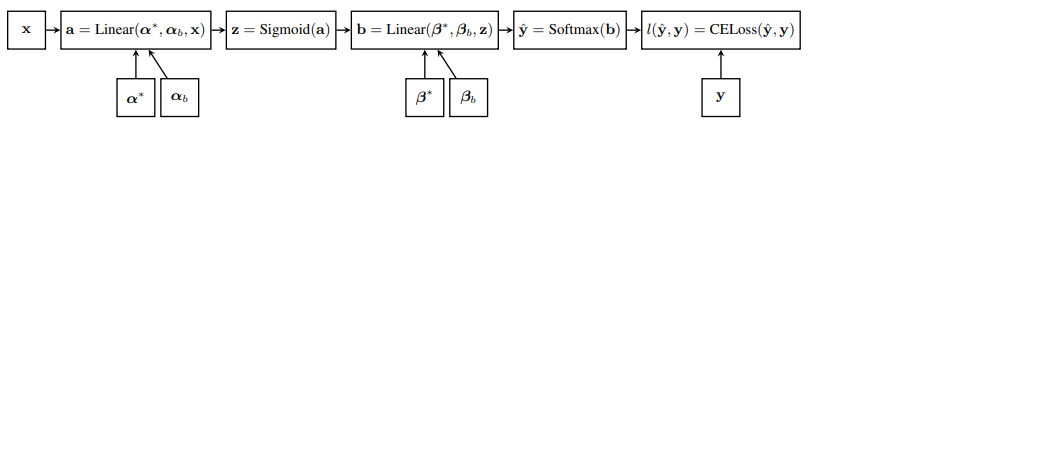
\includegraphics[scale = 0.7]{images/sg5 diagram.png}
% % \end{rightjustify}
% % \centering
% \vspace{-5.5cm}
% %\hspace{2cm}
% \caption{Computational Graph from CMU \textit{Introduction to Machine Learning} assignment}
% %\end{rightjustify}
% \label{fig: NN}
% %\vspace{-0.7cm}
% %\end{wrapfigure}
% \end{figure}
%\vspace{1cm}
\subsection{\textit{Medical Device Innovation and Realization: 42-678}}
This class revolved around a project as well as covering the FDA approval process and standards. My group's project was an improved cell encapsulation device-- one based off of Viacyte inc. that is made of ePTFE(stretched Teflon) (Figure \ref{fig: viacyte}). My contributions to the group were my COMSOL simulations and Solidworks designs that were based on my group's drawings (Figure \ref{fig: solidworks}). We saw in the literature \cite{Yang} an optimized geometry that would increase encapsulated cell viability and simulated the resulting increased diffusion of oxygen. I also 3D printed our design at 2:1 scale (Figure \ref{fig: 3d image}).

%\newcounter{MDIR_width}{1.0}
%\begin{SCfigure}[1.0][h]
\begin{figure}[h]
%\begin{wrapfigure}{r} {0.5\textheight}
\vspace{-1cm}
%\sidecaptionsep{1.0}
%
\includegraphics[scale = 0.6]{portfolio images.png}
%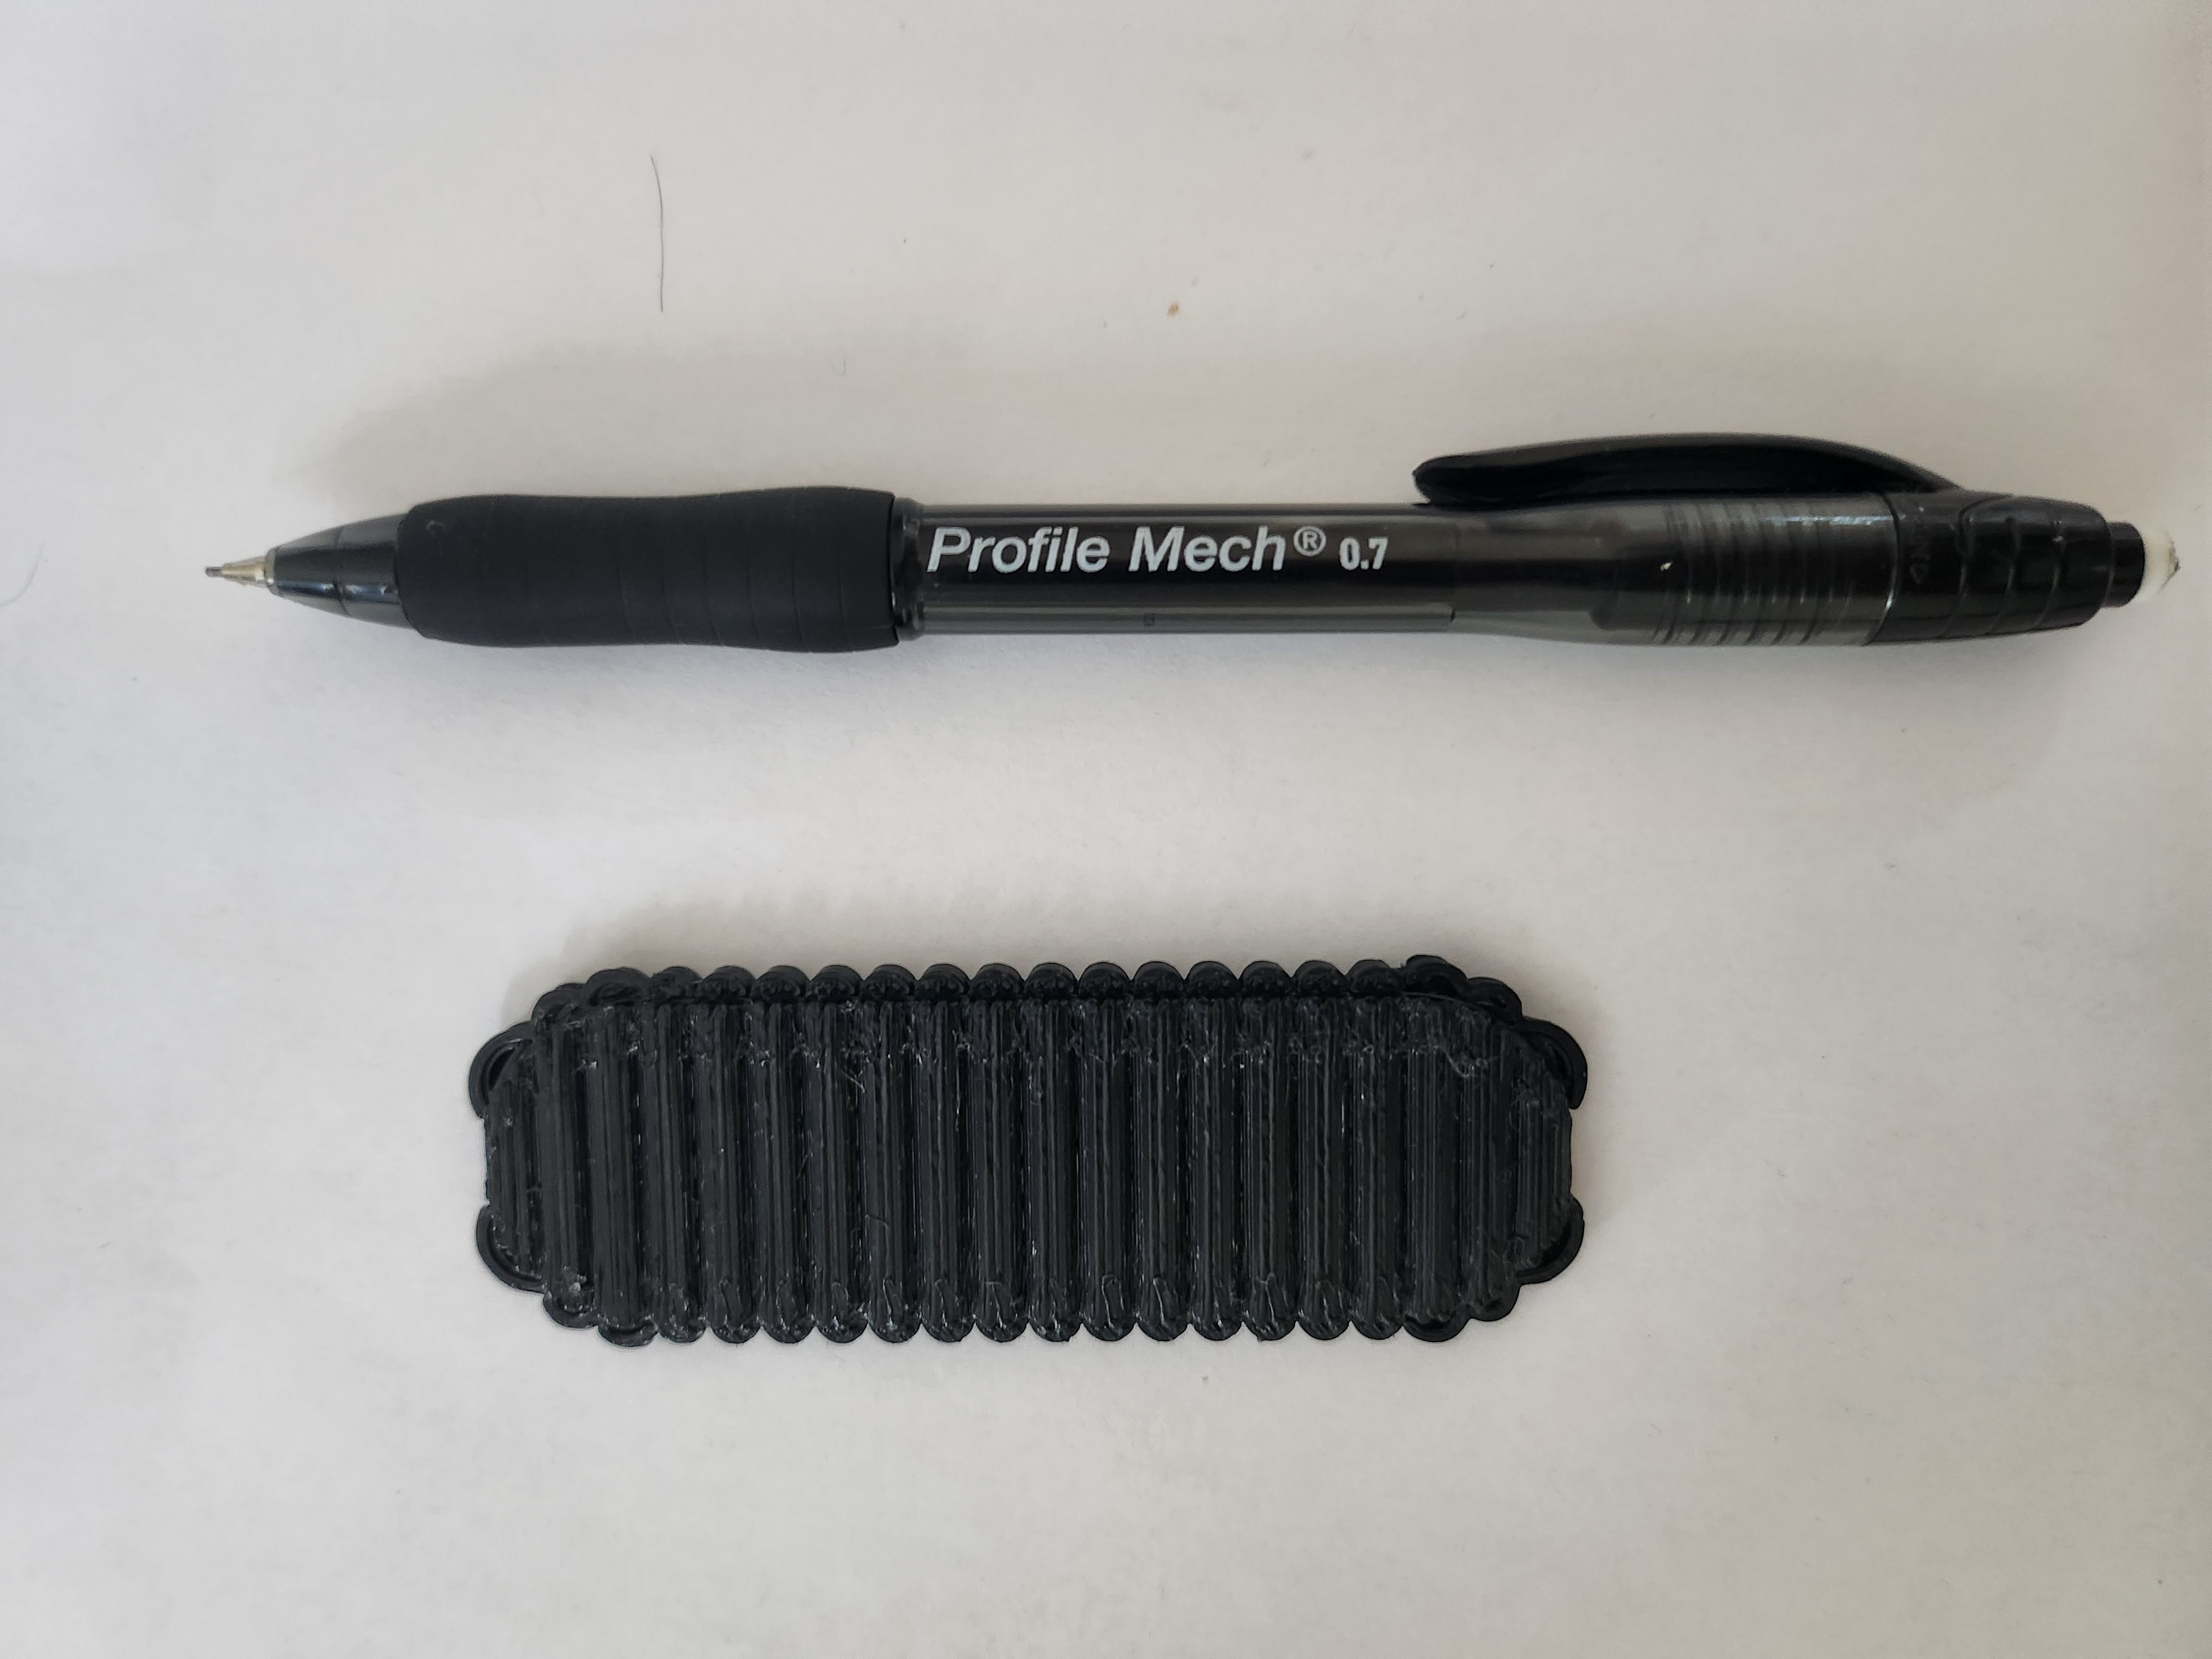
\includegraphics[height=4cm]{images/20230428_124536.jpg}
\begin{subfigure}[t][10pt][t]{0.5\textwidth}
%\vspace{-1cm}
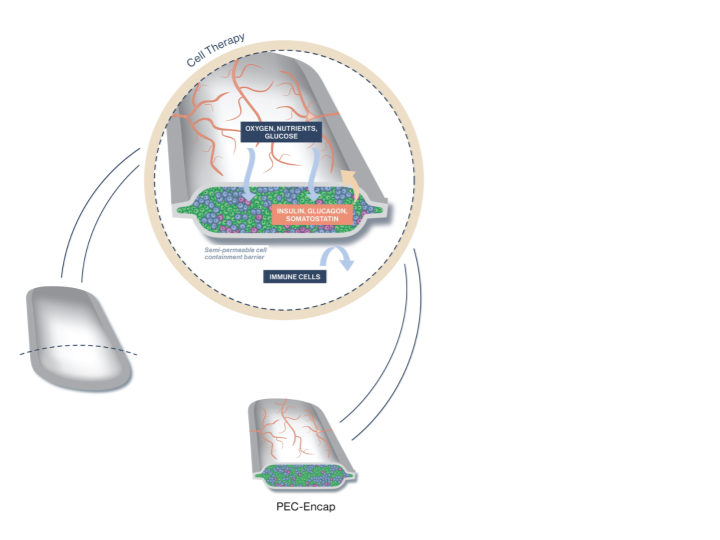
\includegraphics[trim={0 0 10cm 0}, clip, scale = 0.5]{images/viacyte image.png}
%\vspace{-1.0cm}
\caption{Promotional material of Viacyte PEC-Encap from Viacyte website depicting transplanted cell protection from host immune cells.}
\label{fig: viacyte}
\vspace{1.0cm}
\end{subfigure}
%https://latex-tutorial.com/subfigure-latex/
%\begin{subfigure}[t][3pt][t]{0.4\textwidth}
%https://www.reddit.com/r/LaTeX/comments/ps5e9i/stacking_subfigures_in_latex/
\hspace{0.5cm}
\begin{minipage}[b]{0.3\textwidth}
%\begin{subfigure}[t][3pt][t]{0.4\textwidth}
\subfloat[\textit{Solidworks} image of geometry-optimized\\ design with measurements in centimeters]{
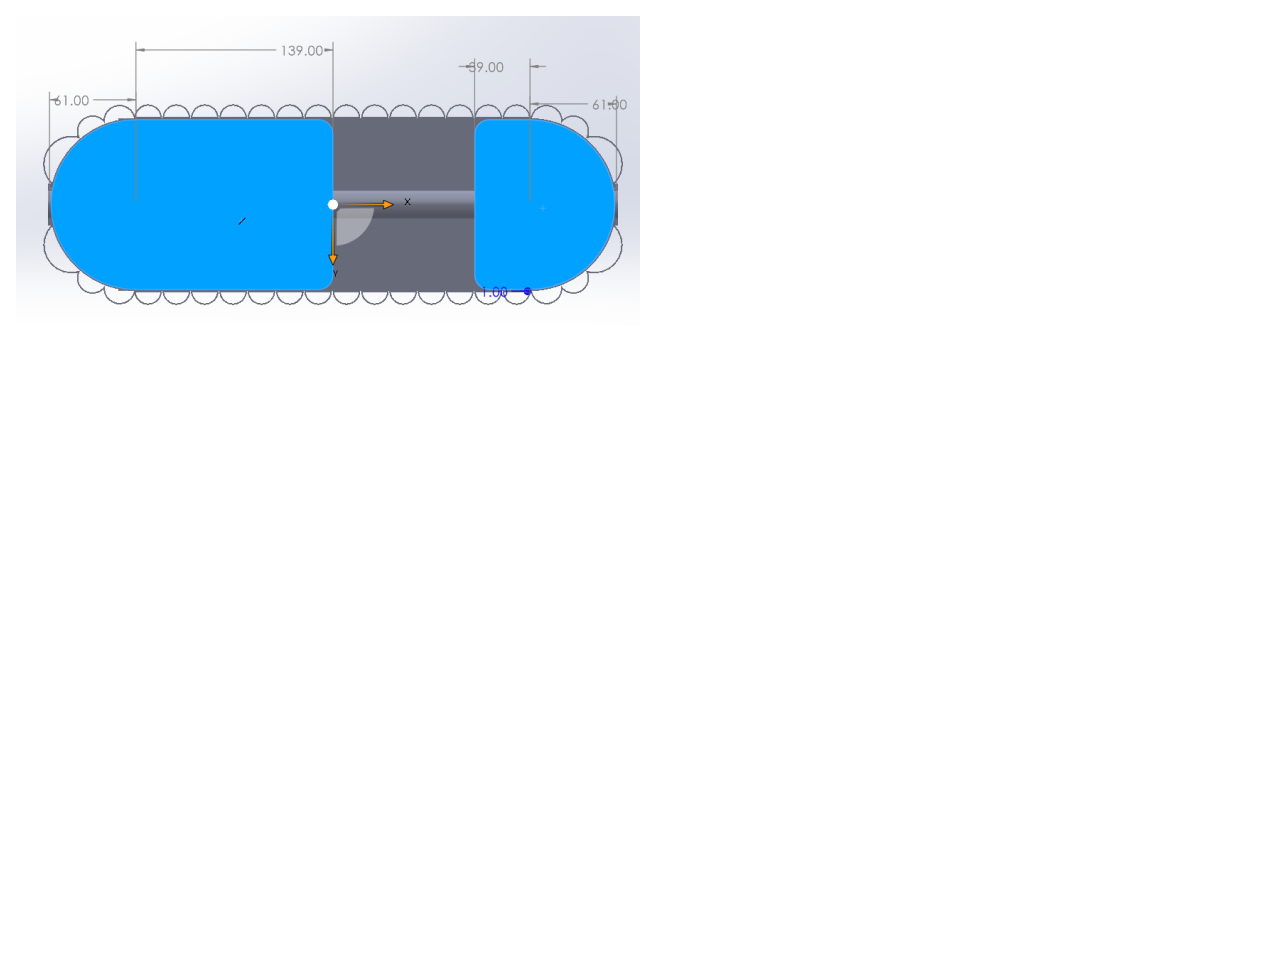
\includegraphics[trim={0 0 10cm 0}, clip, scale = 0.3]{images/portfolio images.png}
\vspace{-7cm}
%\caption{\textit{Solidworks} image of geometry-optimized design with measurements in cm}
\label{fig: solidworks}
}
%\end{subfigure}
%\hspace{10cm}
\hfill
%\begin{subfigure}[b][3pt][b]{0.2\textwidth}
\subfloat[Top-down view of 3D-printed version of geometry-optimized design with pen for reference]{
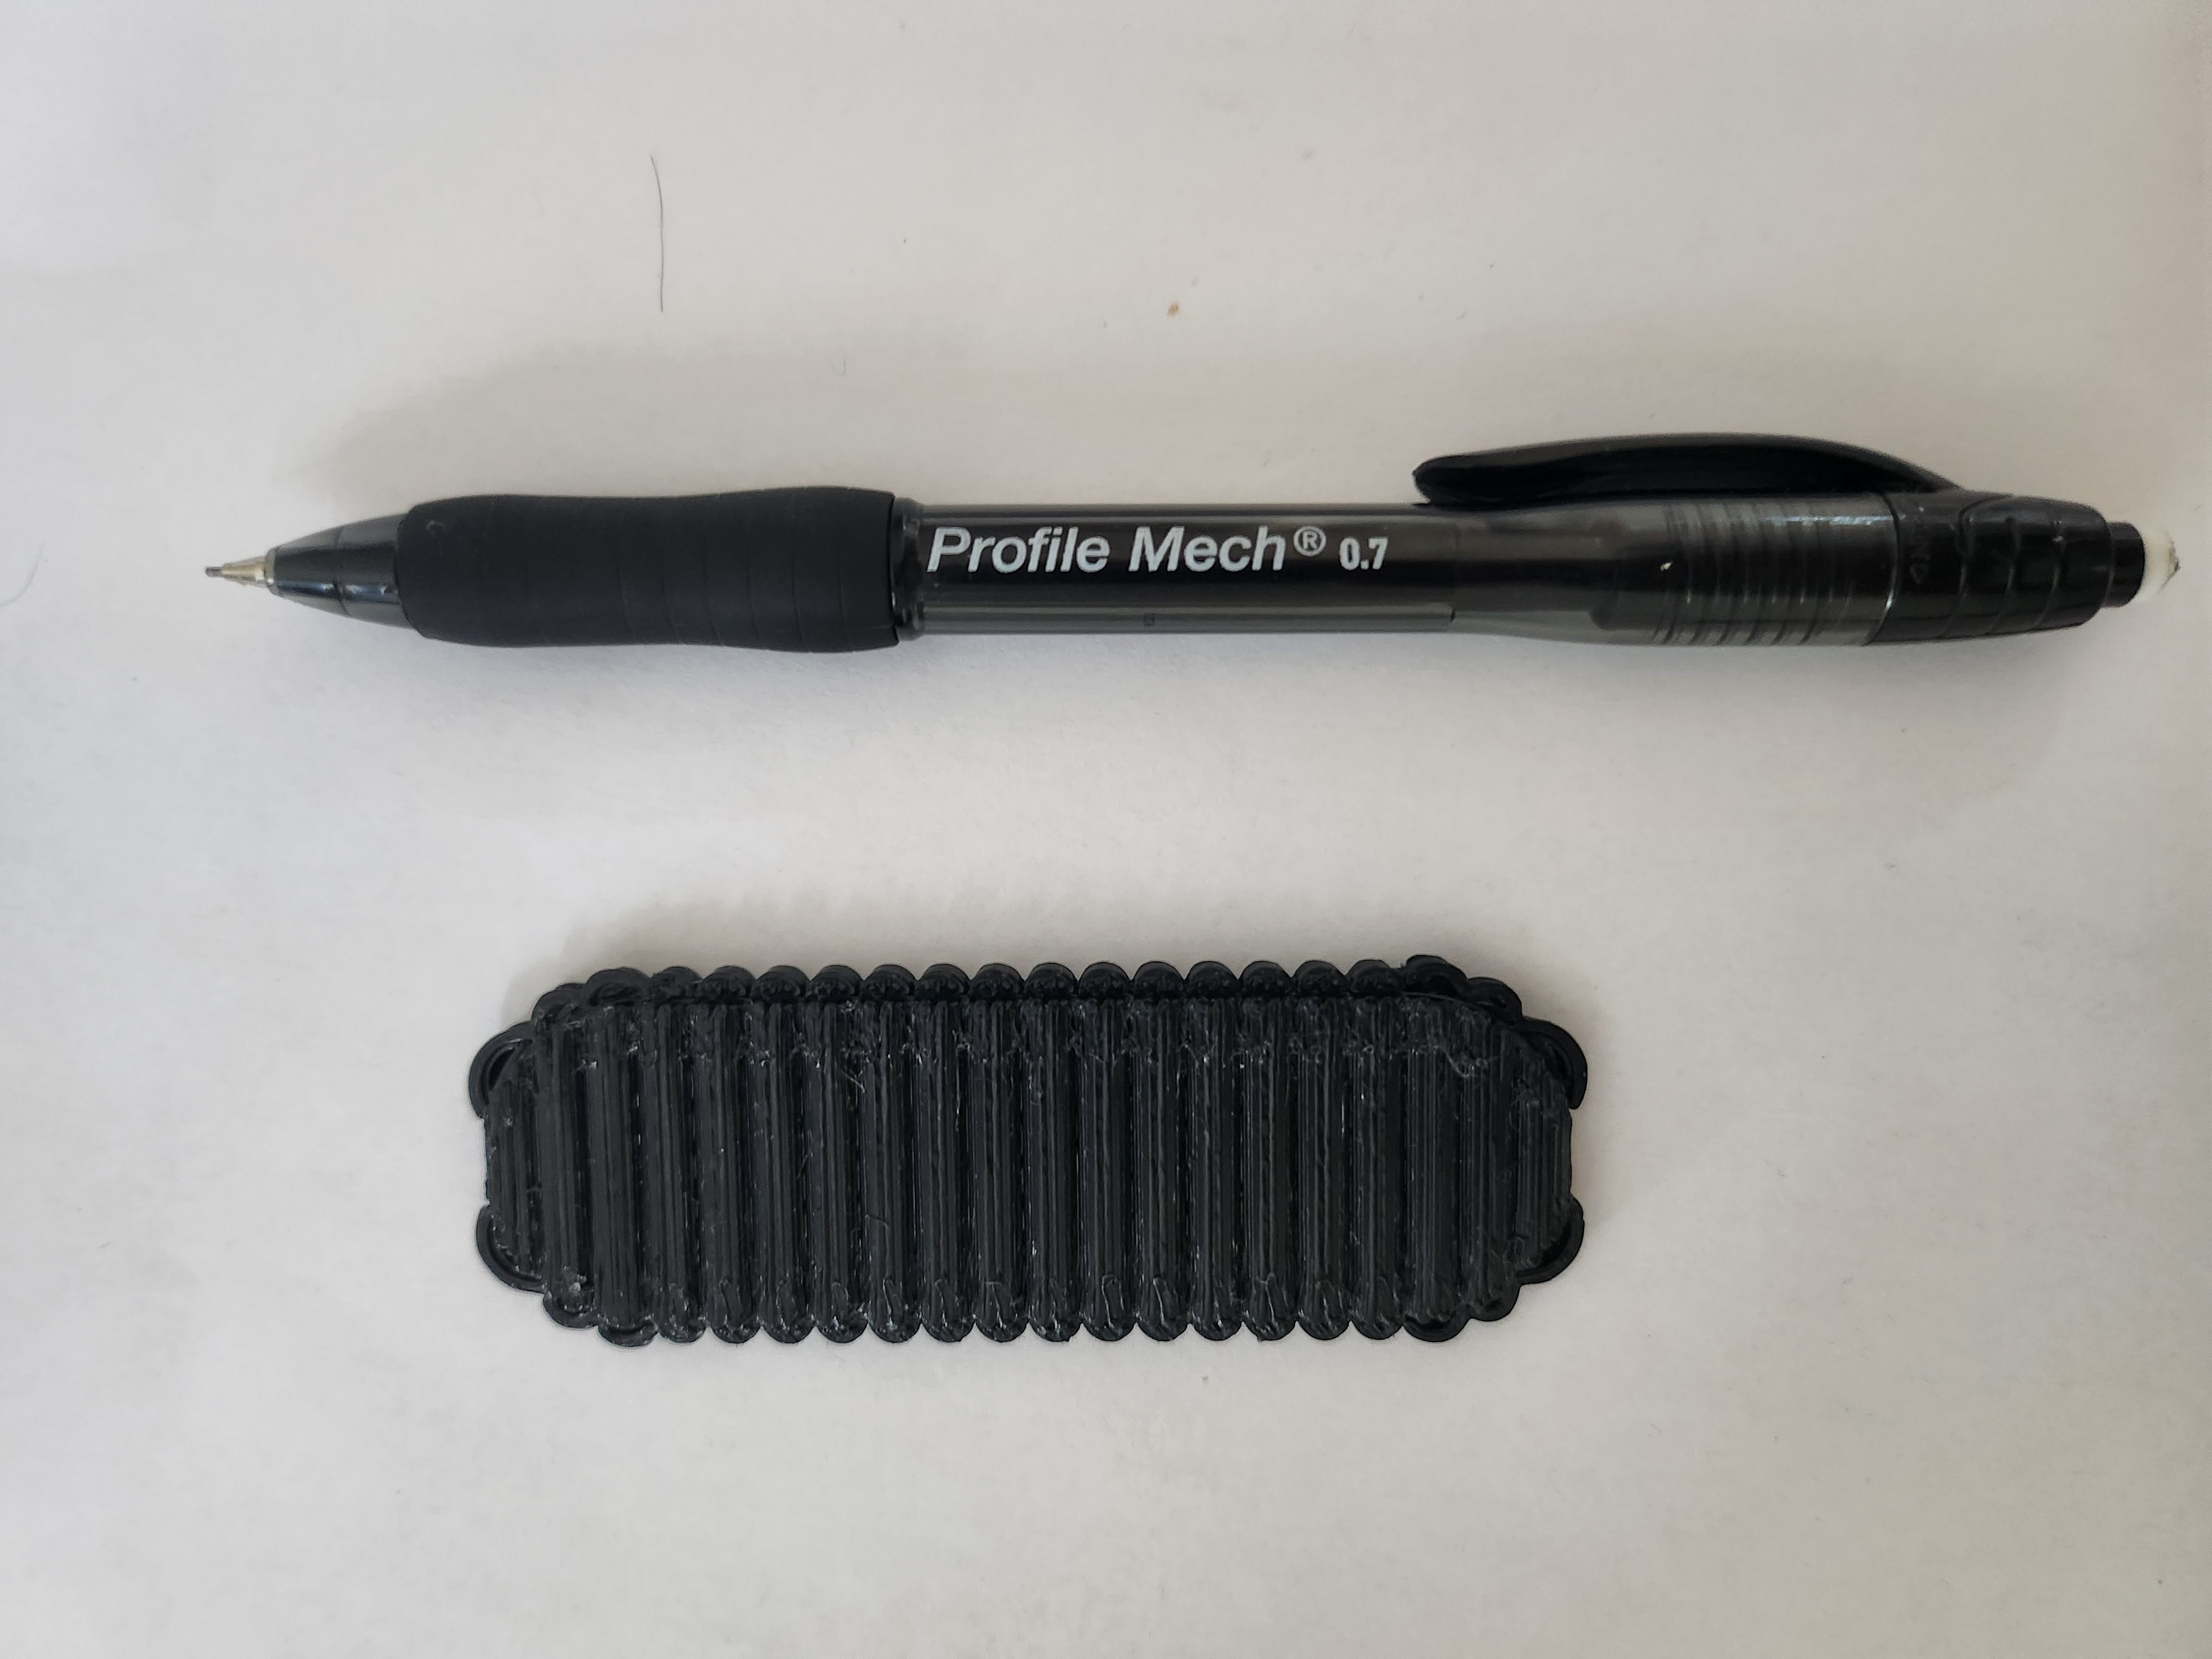
\includegraphics[height=5cm]{images/20230428_124536.jpg}
%\caption{top-down view of 3D-printed version of geometry-optimized design with pen for reference}
\label{fig: 3d image}
}
%\end{subfigure}
\end{minipage}
\caption{Images depicting my group's \textit{Medical Device Innovation
and Realization} project from inspiration (\ref{fig: viacyte}), to CAD model (\ref{fig: solidworks}), followed by 3D print (\ref{fig: 3d image}). }
% \vspace{1.0cm}
\end{figure}
%\vspace{-2.5cm}
%\end{SCfigure}
%\end{wrapfigure}
% \newpage
\subsection{\textit{Micro/Nano Biomedical Devices: 42-693}}
% \vspace{1cm}
% \begin{wrapfigure}[40]{r} {0.38\textwidth}

This class covered the principles behind biomedical devices that interacted with the micro- and/or nano-scale such as microfluidics and fabrication. I learned about electrokinetic flows and gained a deeper understanding of bioelectrical phenomena. COMSOL was used as a teaching tool in this course-- with one such digital laboratory figure being depicted in Figure \ref{fig: elec}. As part of my final group project, a fellow PhD student and I iterated on her Master's thesis looking at the gradual release of a niosome-coated dental implant.
\begin{figure}[h!]
%\hspace{-2cm}
% \vspace{-1.5cm}
%\fbox{
%
\includegraphics[scale = 0.5]{Electro-Osmotic Mircomixer Concentration Profile.png}
\centering
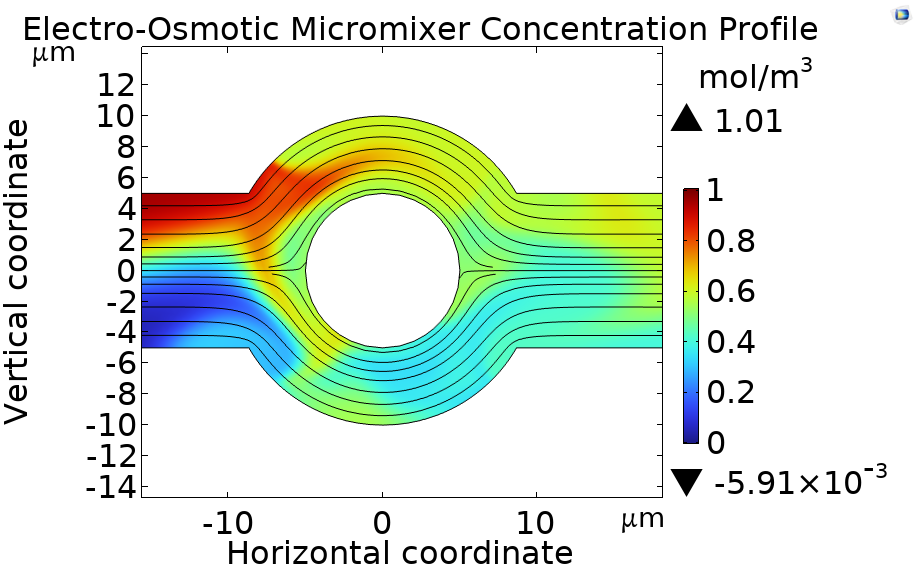
\includegraphics[clip, scale = 0.4]{images/Electro-Osmotic Mircomixer Concentration Profile.png}
%\vspace{-0.3cm}
% \vspace{-3cm}
%\hspace{2cm}
%\fbox{
%\begin{framed}
%\begin{tcolorbox}
\caption{COMSOL plot of a 2D steady-state electro-osmotic micromixer depicting concentration profile of a generic solute}
%\end{framed}
%\end{tcolorbox}
\label{fig: elec}
% \vspace{-1cm}
% \end{wrapfigure}
\end{figure}
\vspace{1cm}

\newpage

\section{Post-Bach research at the University of Minnesota's Department of Mechanical Engineering}
During the COVID-19 pandemic, I was offered the opportunity to research improvements for a COVID-19 rapid diagnostic reader at the University of Minnesota in John Bischof's group. Dr. Bischof's BioHeat and Mass Transfer (BHMT) group specializes in the thermodynamics of colloidal solutions-- the applications of this research being in areas like cryopreservation and point-of-care diagnostics.

% \subsection{Introduction}
\subsection{Thermal Contrast Amplification Diagnostic Test Reader}

%\parindent 
Thermal contrast amplification (TCA) is a technology platform to improve rapid diagnostics, specifically lateral flow assays (LFAs). Previous BHMT researchers developed this device wherein regions of concentrated gold nanosphere deposits are plasmonically resonated by a moving, 532 nm-wavelength laser to emit heat that is picked up by an IR camera as it and the laser move across the test strip, like the still image depicted in Figure \ref{fig: tca}.

\begin{wrapfigure}[14]{rt} {0.4\textwidth}
\vspace{-2.5cm}
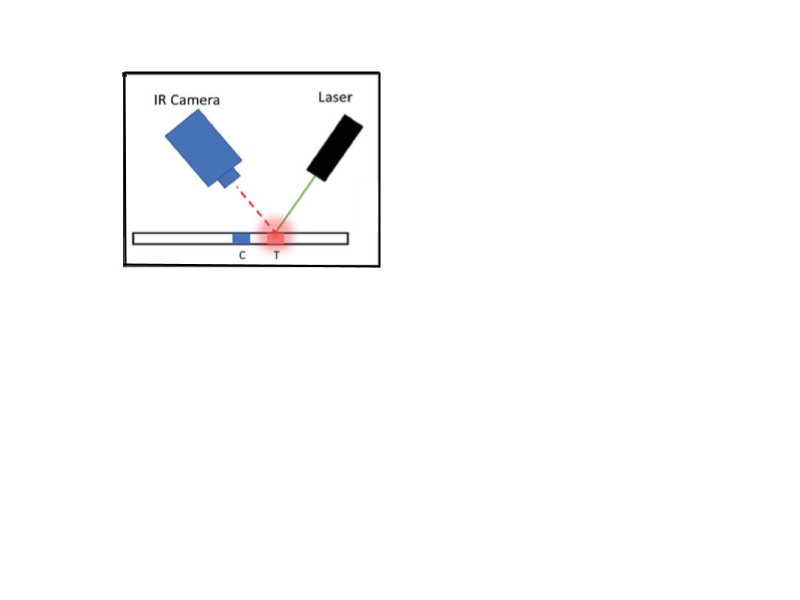
\includegraphics[trim={4cm 0 1cm 0},clip, scale = 0.7]{images/TCA diagram.png}
\vspace{-9cm}
% \parbox{4cm}{
\caption{Schematic for thermal contrast amplification (TCA) focused on the lateral flow assay (LFA) test line (T). Figure snippet from reference \cite{Wang}\label{fig: tca}}
% \vspace{-5cm}
\vfill
\end{wrapfigure}

My initial contributions included making the lateral flow assays being scanned for reading. This process entailed gold nanoparticle (GNP) preparation and synthesis as well as assisting with the specialized dispenser and an automatic cutting paper-cutter. GNP synthesis using the citrate method included characterization with dynamic light scattering (DLS) and spectrophotometry. I would also conjugate antibodies to the GNP I synthesized for use in the testing solution we would run. This testing solution involved buffer selection and optimization to ensure proper antibody binding while minimizing aggregation of the GNPs.

For my third-author publication \cite{Liu} I developed the antibody binding site assay. Briefly, this involved a buffer exchange to set up an off-the-shelf protein crosslinking reaction so I could then use a plate reader to make comparisons between antibody-GNP solutions. My goal was to crosslink antigen and marker molecule with a cleavable bond so that we could assess binding site availability across the industry standard of physical conjugation with our group's covalent conjugation (Figure \ref{fig: rpe-dtt}).
% \newpage
%\\Going through the entire synthesis process: \\
% \noindent
% \hfill{
% \makebox[\textwidth]{
% \restoregeometry

\begin{figure}[ht] 
%{0.4\textwidth}
\vspace{-1cm}
% \hspace{6cm}
\begin{center}
\hspace{2cm}
\justifying{
\adjincludegraphics[trim={0 0 5cm 0}, clip, scale = 0.5]{images/Liu R-PE dtt figures.png}}
\end{center}
\vspace{-10cm}
\caption{Schematic of antigen binding site characterization using PE(phycoerythrin)-antigen conjugate for conjugated gold nanospheres (GNS). Edited figure snippet from reference \cite{Liu}}
%\vspace{-1cm}
\label{fig: rpe-dtt}
\end{figure}

Another consideration of the antibody binding site assay was calculating a molar availability. I was in the process of testing polyacrylamide gel electrophoresis (PAGE) to determine the conjugation ratio of the flourophore-antigen conjugate I synthesized before shifting priorities. The major consideration was that sodium dodecyl sulfate in conventional SDS-PAGE would cleave the disulfide bond in the conjugate, hence I would need to test and select reagents with that in mind.

% \begin{wrapfigure}[17]{r} {0.4\textheight}
\begin{figure}[h]
\centering
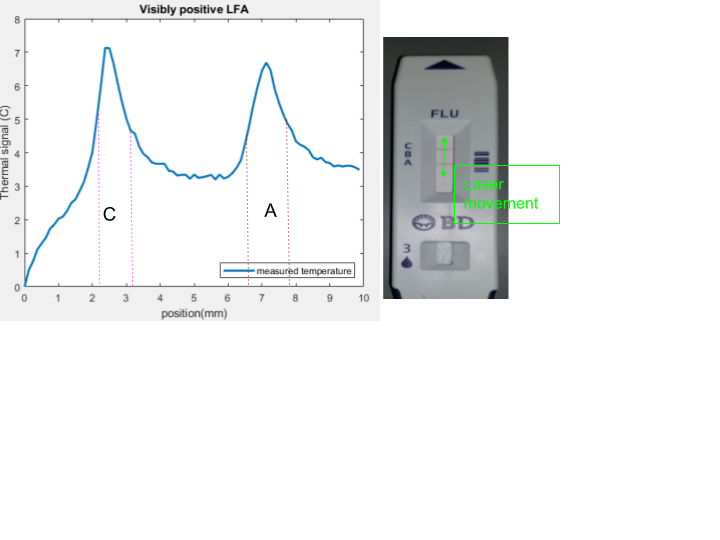
\includegraphics[trim={0 2cm 5cm 0}, clip, scale = 0.5]{images/TCA peaks.png}
\vspace{-2.5cm}
\caption{Side-by-side comparison of thermal readout with laser positioning on the LFA. Thermal signal is a calculation of the IR camera's reading of the laser region subtracted from an established baseline background.}
\label{fig: peaks}
% \vspace{-1cm}
% \end{wrapfigure}
\end{figure}

Computing test determinations following a run was another aspect to the TCA reader. Because regions of high GNP deposition readily heat upon laser exposure, a spike in measured temperature corresponds to antibody binding at the line regions of the LFA (Figure \ref{fig: peaks}). 
%\vspace{-0.5cm}

The specific interests we have in test determination are (a) long stretches of a rise in temperature-- this could correspond to the dispensed line of interest on the LFA and is therefore less likely to be noise-- and (b) large increases-- to indicate the aforementioned deposits of antibody-GNP binding. These interests lead to the selection of a sort of area-under-the-curve (AUC) is used. Where a threshold AUC value for positive tests is determined from a dataset of control tests. The actual calculation is more of an average-under-the-curve where, \begin{center}
\begin{equation} \label{eqn1}
AUC=mean(\Delta T)
\end{equation}
\begin{equation} \label{eqn2}
\Delta T = T(A_{start}:A_{end})-T_{background}
\end{equation}
\end{center} 

With $AUC$ being the average temperature, $\Delta T$, (Equation \ref{eqn1}) across a defined interval of positions $A_{start}:A_{end}$, (Equation \ref{eqn2}) i.e. indices in the $T$ vector, subtracted by a calculated background temperature, $T_{background}$. In the 1.0 version I wrote for the publication \cite{Liu}, I calculated $T_{background}$ from averaging a few points left of $A_{start}$ and a few points right of $A_{end}$. %The chief concern in analyzing a given temperature readout is therefore properly defining $A_{start}:A_{end}$. 
The interval $A_{start}:A_{end}$ represents the test line of the LFA where antibody-GNP binding is expected to occur. This interval is easily estimated by using positive control LFAs to measure out intervals and recording the TCA readout. My 1.0 version was also designed around a generous estimate for human error in physical test placement via a search for the maximum rolling average within a wider interval. These improvements combined with Excel-to-Matlab cross-communication functions I found and added to the code made data processing much more automated, hence a more than 50\% reduction in processing times.

The 2.0 version of the TCA test determination algorithm was designed by the chief technical officer of VigilantDx-- the startup for this test reader. His implementation added a consideration of the control line into the calculations as well as an efficient linear regression for background calculation (Figures \ref{fig: overarching}, \ref{fig: CL}, and \ref{fig: TL}). 

\begin{figure}[h!] 
\begin{center}
%\centering
\subfloat[Summary diagram of test determination algorithm]{
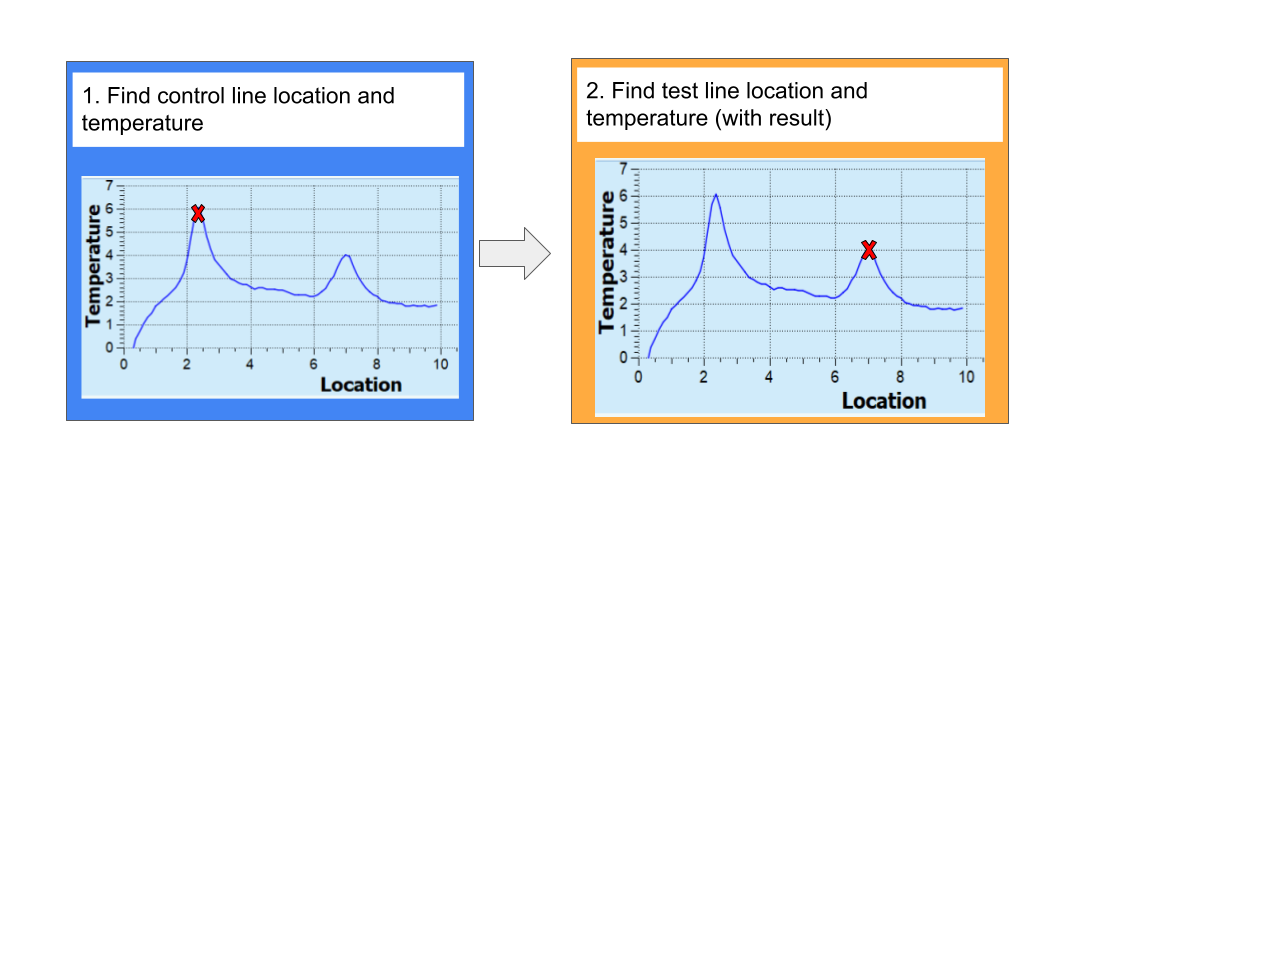
\includegraphics[clip, scale = 0.3]{images/TCA logic a.png}
\vspace{-5.5cm}
\label{fig: overarching}
%\vspace{1.0cm}
}
\end{center}
% \caption{Piecewise flowchart of TCA test determination algorithm version 2.0}
% \label{fig: logic}
% \end{figure}

% \newpage

% \begin{figure}[h!] 
% \ContinuedFloat
\vspace{-1cm}
%\hspace{0.5cm}
%\begin{minipage}[b]{\textwidth}

%\hfill
\begin{center}
\subfloat[Detailed process for control line location]{
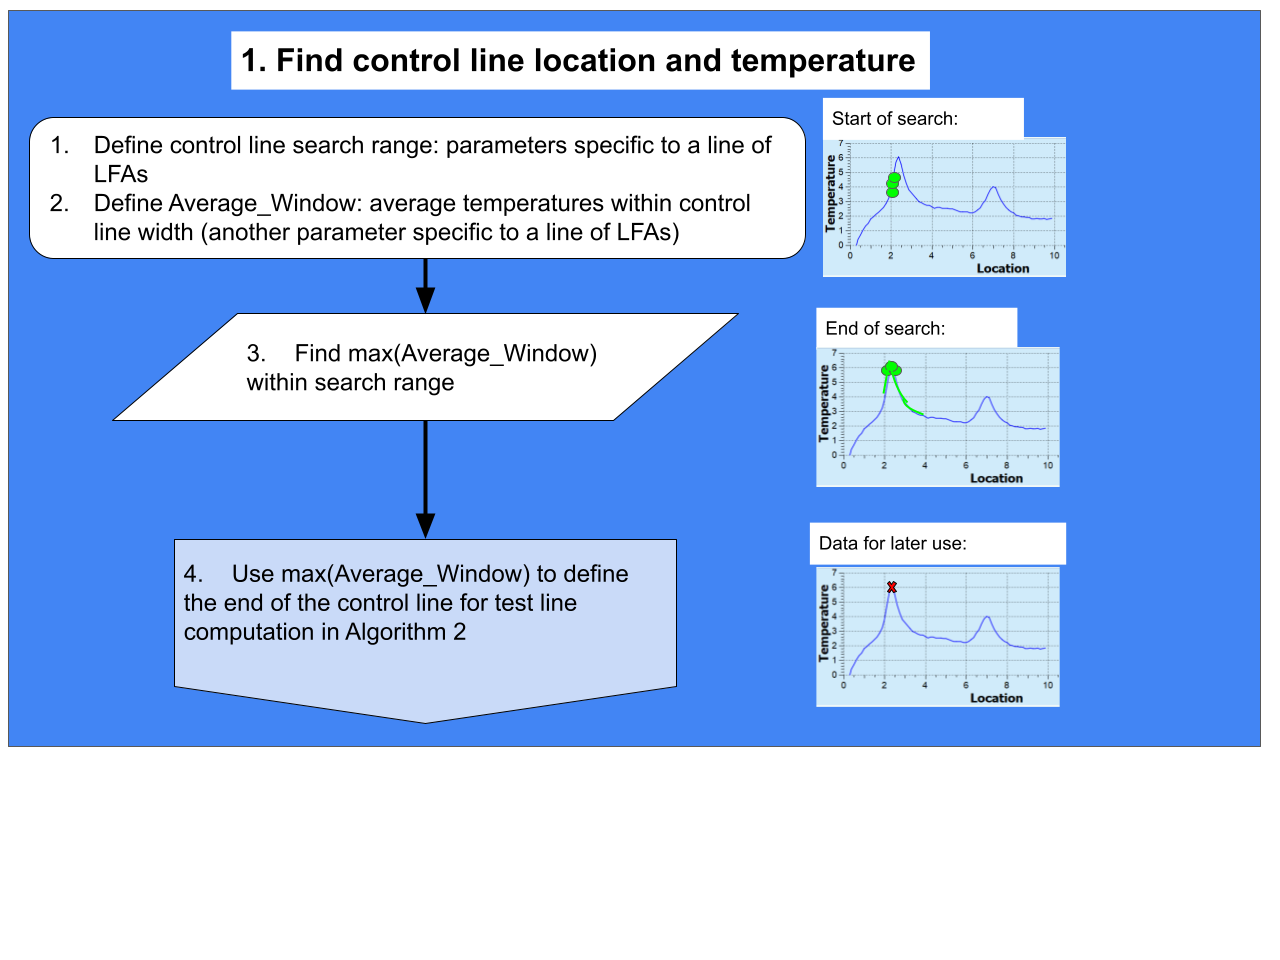
\includegraphics[clip, scale = 0.3]{images/TCA flowchart b.png}
\vspace{-2cm}
\label{fig: CL}
}
%\end{subfigure}
%\hspace{10cm}
\end{center}
\begin{center}
\subfloat[Detailed process for final test determination]{
%\vspace{1cm}
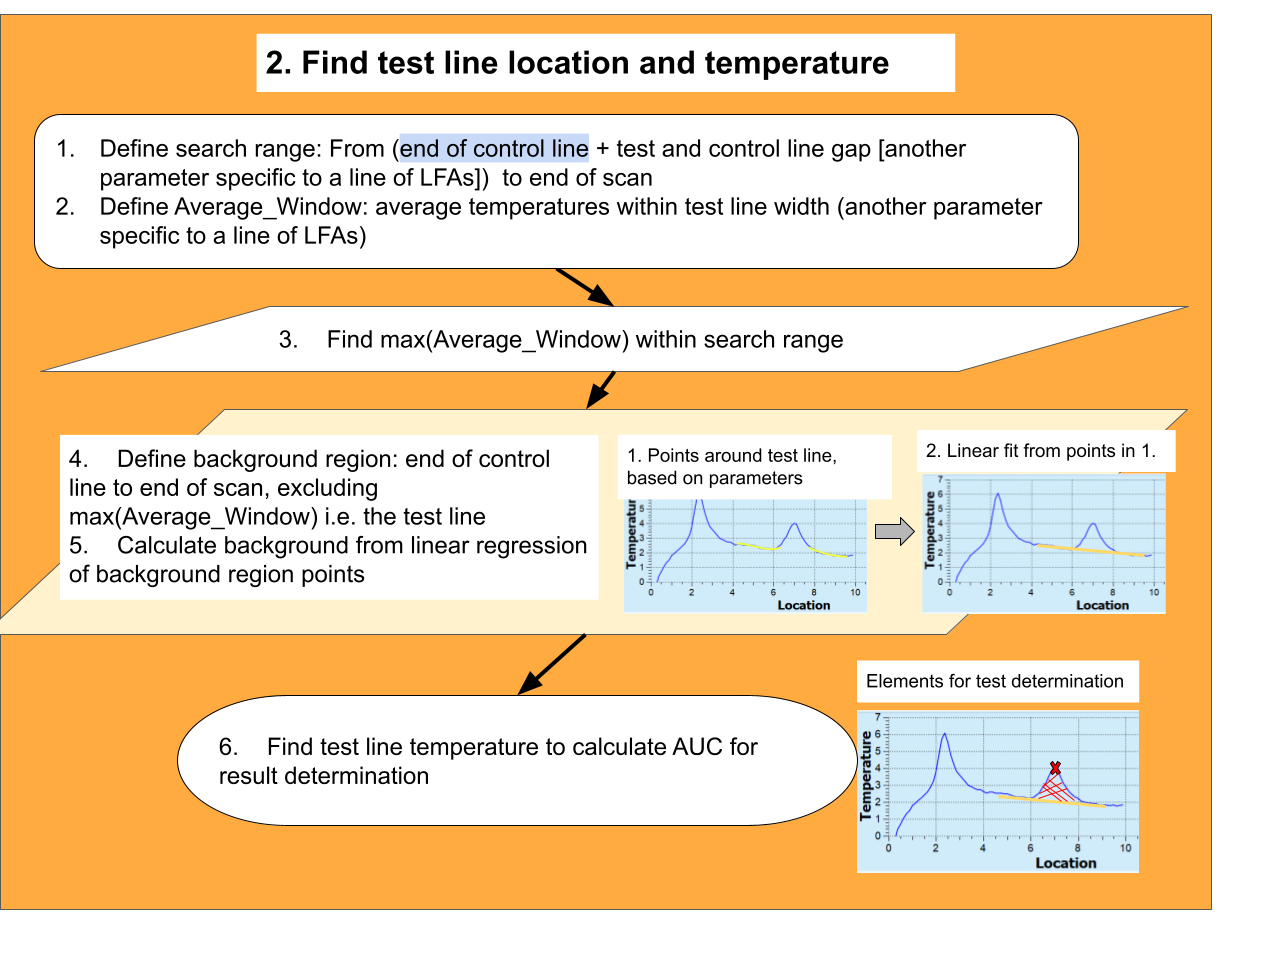
\includegraphics[scale = 0.3]{images/TCA flowchart c.png}
\label{fig: TL}
%\vspace{-1cm}
}
\vspace{-0.5cm}
\end{center}
% \vspace{-1cm}
\caption{Piecewise flowchart of TCA test determination algorithm version 2.0}
\hfill
%\begin{subfigure}[b][3pt][b]{0.2\textwidth}

\hfill
\label{fig: logic1}
\vspace{-1cm}
\end{figure}
%%% If ending here instead of with aquaculture: %%%

% The remainder of my duties involving the TCA reader were validation tests with the 2.0 algorithm and device hardware itself. This project became my primary focus before going on to Carnegie Mellon University for graduate school, I trained my replacement and also wrote and produced instructional manuals and videos for the reader and GNP synthesis.

% \newpage
% \subsection{Aquatic Species Cryopreservation}
% Among the other projects of the BHMT group, I was also involved with the cryopreservation of zebrafish embryos. Building off of previous successes of whole zebrafish embryo cryopreservation in the group \cite{Khosla}, we sought to improve primordial germ cell (PGC) cryopreservation with the procedures used in previous work. PGC cryopreservation allows for a simpler target for vitrification and can easily be transplanted in other fish for efficient husbandry \cite{higaki}-- equivalent to cryopreserving whole embryos if not potentially moreso. \\

% Once I was proficient in microinjection, a key consideration was removing the yolk from the embryo which I had built using parts already available in the research space (Figure \ref{fig: microyolk}). Difficulties in producing a GFP-plasmid for PGC tagging with collaborators kept this project on indeterminate hold and my results with the yolk extractor were purely preliminary before I had to move on. I believe the core parts were adaptable and did not require the exceptional handling required in the previous work's supplemental video \cite{higaki} with fine-tuning primarily for the long-tipped (LT) pipette.
% \newpage
% \vspace{4cm}
% % \begin{figure}[h]
% % \begin{center}
% % \hspace{10cm}
% % \fcapside
% % % \captionsetup[capbesidefigure]
% % %{justification=raggedright}%
% % \thisfloatsetup{capbesideposition=right}
% % % [\FBwidth]
% % % [t]
% % {\caption{Diagram for building a zebrafish yolk extractor from available magnetic microinjection setup.\label{fig: microyolk}}}
% % {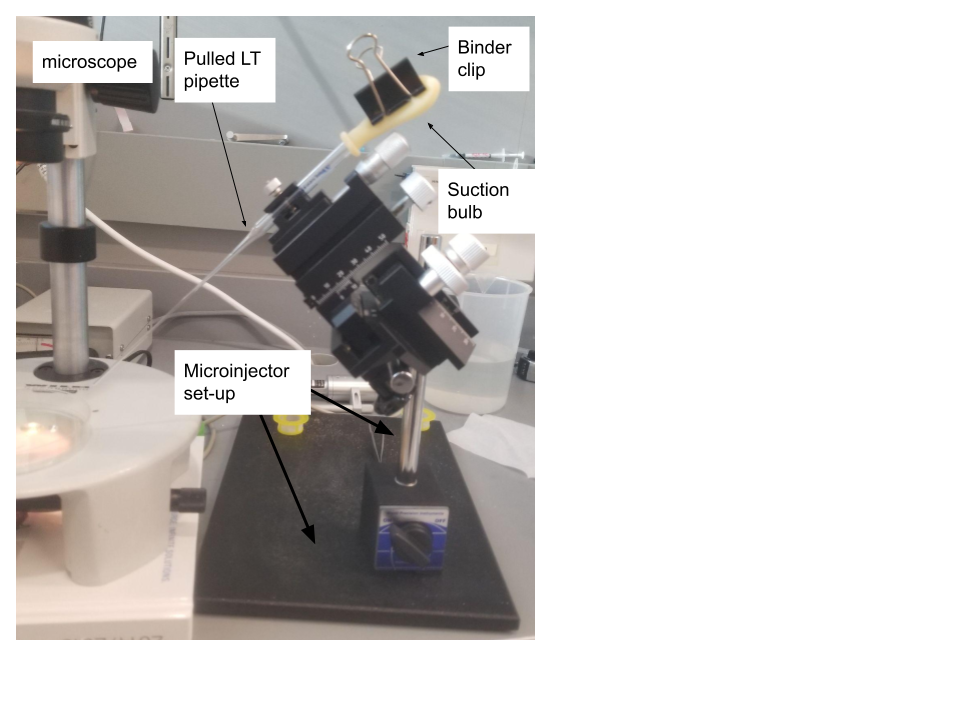
\includegraphics[right, scale = 0.4]{images/Yolk Extraction_embryo digestion.png}}
% % % \end{center}
% % \end{figure}
% % \vspace{4cm}
% \begin{SCfigure}[50][h]
% \vspace{-1cm}
%     % \begin{center}
%     % \justifying{
%     \hspace{2cm}
%     \vspace{5cm}
%     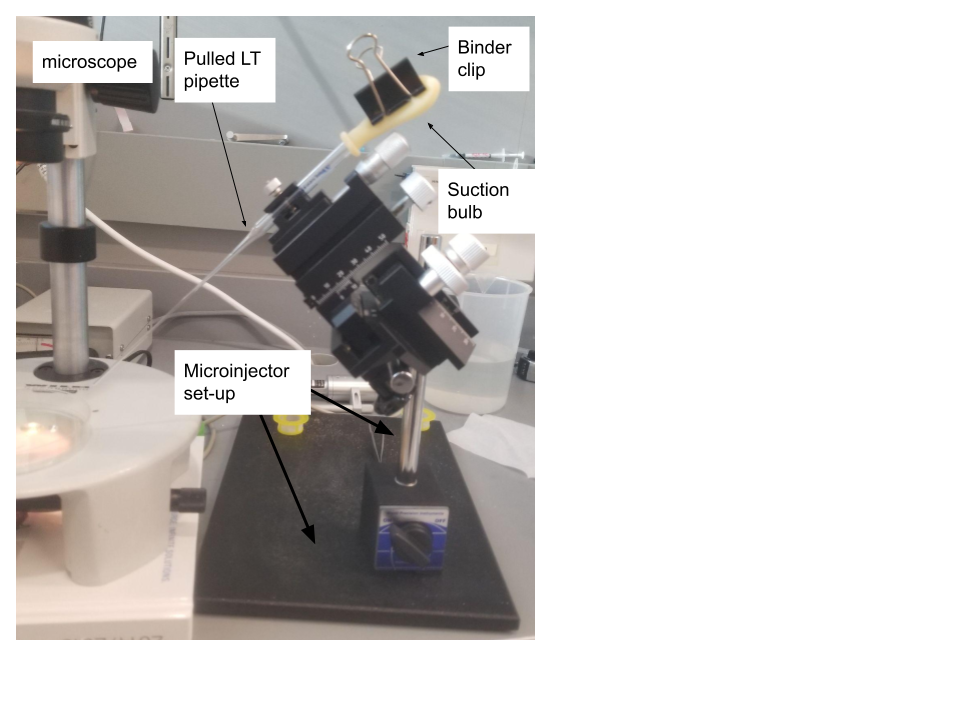
\includegraphics[trim={0 0 15cm 0}, clip, scale = 0.4]{images/Yolk Extraction_embryo digestion.png}    
%         \vspace{-5cm}
%     % \hspace{-8cm}
%     \caption{Diagram for building a zebrafish yolk extractor from available magnetic microinjection setup.}
% \label{fig: microyolk}
%     % \end{center}
%     % \vspace{5cm}
% \end{SCfigure}
% During the COVID-19 pandemic, I was offered the opportunity to research improvements for a COVID-19 rapid diagnostic reader at the University of Minnesota in John Bischof's group. Dr. Bischof's BioHeat and Mass Transfer (BHMT) group specializes in the thermodynamics of colloidal solutions-- the applications of this research being in areas like cryopreservation and point-of-care diagnostics.

% % \subsection{Introduction}
% \subsection{Thermal Contrast Amplification Diagnostic Test Reader}

% %\parindent 
% Thermal contrast amplification (TCA) is a technology platform to improve rapid diagnostics, specifically lateral flow assays (LFAs). Previous BHMT researchers developed this device wherein regions of concentrated gold nanosphere deposits are plasmonically resonated by a moving, 532 nm-wavelength laser to emit heat that is picked up by an IR camera as it and the laser move across the test strip, like the still image depicted in Figure \ref{fig: tca}.

% \begin{wrapfigure}[14]{rt} {0.4\textwidth}
% \vspace{-2.5cm}
% 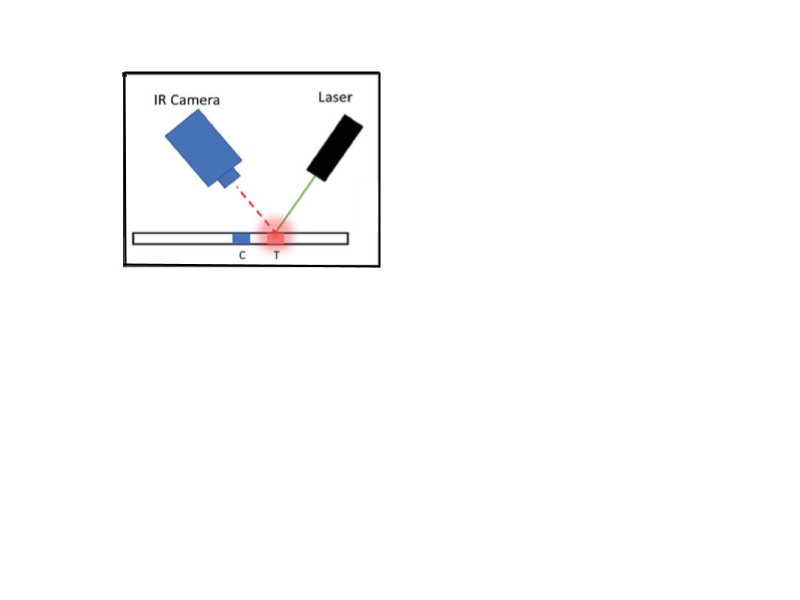
\includegraphics[trim={4cm 0 1cm 0},clip, scale = 0.7]{images/TCA diagram.png}
% \vspace{-9cm}
% % \parbox{4cm}{
% \caption{Schematic for thermal contrast amplification (TCA) focused on the lateral flow assay (LFA) test line (T). Figure snippet from reference \cite{Wang}\label{fig: tca}}
% % \vspace{-5cm}
% \vfill
% \end{wrapfigure}

% My initial contributions included making the lateral flow assays being scanned for reading. This process entailed gold nanoparticle (GNP) preparation and synthesis as well as assisting with the specialized dispenser and an automatic cutting paper-cutter. GNP synthesis using the citrate method included characterization with dynamic light scattering (DLS) and spectrophotometry. I would also conjugate antibodies to the GNP I synthesized for use in the testing solution we would run. This testing solution involved buffer selection and optimization to ensure proper antibody binding while minimizing aggregation of the GNPs.

% For my third-author publication \cite{Liu} I developed the antibody binding site assay. Briefly, this involved a buffer exchange to set up an off-the-shelf protein crosslinking reaction so I could then use a plate reader to make comparisons between antibody-GNP solutions. My goal was to crosslink antigen and marker molecule with a cleavable bond so that we could assess binding site availability across the industry standard of physical conjugation with our group's covalent conjugation (Figure \ref{fig: rpe-dtt}).
% % \newpage
% %\\Going through the entire synthesis process: \\
% % \noindent
% % \hfill{
% % \makebox[\textwidth]{
% % \restoregeometry

% \begin{figure}[ht] 
% %{0.4\textwidth}
% \vspace{-1cm}
% % \hspace{6cm}
% \begin{center}
% \hspace{2cm}
% \justifying{
% \adjincludegraphics[trim={0 0 5cm 0}, clip, scale = 0.5]{images/Liu R-PE dtt figures.png}}
% \end{center}
% \vspace{-10cm}
% \caption{Schematic of antigen binding site characterization using PE(phycoerythrin)-antigen conjugate for conjugated gold nanospheres (GNS). Edited figure snippet from reference \cite{Liu}}
% %\vspace{-1cm}
% \label{fig: rpe-dtt}
% \end{figure}

% Another consideration of the antibody binding site assay was calculating a molar availability. I was in the process of testing polyacrylamide gel electrophoresis (PAGE) to determine the conjugation ratio of the flourophore-antigen conjugate I synthesized before shifting priorities. The major consideration was that sodium dodecyl sulfate in conventional SDS-PAGE would cleave the disulfide bond in the conjugate, hence I would need to test and select reagents with that in mind.

% % \begin{wrapfigure}[17]{r} {0.4\textheight}
% \begin{figure}[h]
% \centering
% 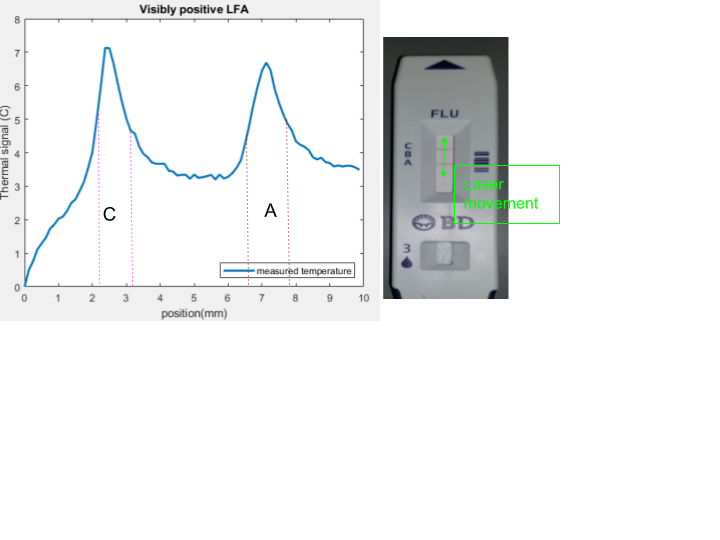
\includegraphics[trim={0 2cm 5cm 0}, clip, scale = 0.5]{images/TCA peaks.png}
% \vspace{-2.5cm}
% \caption{Side-by-side comparison of thermal readout with laser positioning on the LFA. Thermal signal is a calculation of the IR camera's reading of the laser region subtracted from an established baseline background.}
% \label{fig: peaks}
% % \vspace{-1cm}
% % \end{wrapfigure}
% \end{figure}

% Computing test determinations following a run was another aspect to the TCA reader. Because regions of high GNP deposition readily heat upon laser exposure, a spike in measured temperature corresponds to antibody binding at the line regions of the LFA (Figure \ref{fig: peaks}). 
% %\vspace{-0.5cm}

% The specific interests we have in test determination are (a) long stretches of a rise in temperature-- this could correspond to the dispensed line of interest on the LFA and is therefore less likely to be noise-- and (b) large increases-- to indicate the aforementioned deposits of antibody-GNP binding. These interests lead to the selection of a sort of area-under-the-curve (AUC) is used. Where a threshold AUC value for positive tests is determined from a dataset of control tests. The actual calculation is more of an average-under-the-curve where, \begin{center}
% \begin{equation} \label{eqn1}
% AUC=mean(\Delta T)
% \end{equation}
% \begin{equation} \label{eqn2}
% \Delta T = T(A_{start}:A_{end})-T_{background}
% \end{equation}
% \end{center} 

% With $AUC$ being the average temperature, $\Delta T$, (Equation \ref{eqn1}) across a defined interval of positions $A_{start}:A_{end}$, (Equation \ref{eqn2}) i.e. indices in the $T$ vector, subtracted by a calculated background temperature, $T_{background}$. In the 1.0 version I wrote for the publication \cite{Liu}, I calculated $T_{background}$ from averaging a few points left of $A_{start}$ and a few points right of $A_{end}$. %The chief concern in analyzing a given temperature readout is therefore properly defining $A_{start}:A_{end}$. 
% The interval $A_{start}:A_{end}$ represents the test line of the LFA where antibody-GNP binding is expected to occur. This interval is easily estimated by using positive control LFAs to measure out intervals and recording the TCA readout. My 1.0 version was also designed around a generous estimate for human error in physical test placement via a search for the maximum rolling average within a wider interval. These improvements combined with Excel-to-Matlab cross-communication functions I found and added to the code made data processing much more automated, hence a more than 50\% reduction in processing times.

% The 2.0 version of the TCA test determination algorithm was designed by the chief technical officer of VigilantDx-- the startup for this test reader. His implementation added a consideration of the control line into the calculations as well as an efficient linear regression for background calculation (Figures \ref{fig: overarching}, \ref{fig: CL}, and \ref{fig: TL}). 

% \begin{figure}[h!] 
% \begin{center}
% %\centering
% \subfloat[Summary diagram of test determination algorithm]{
% 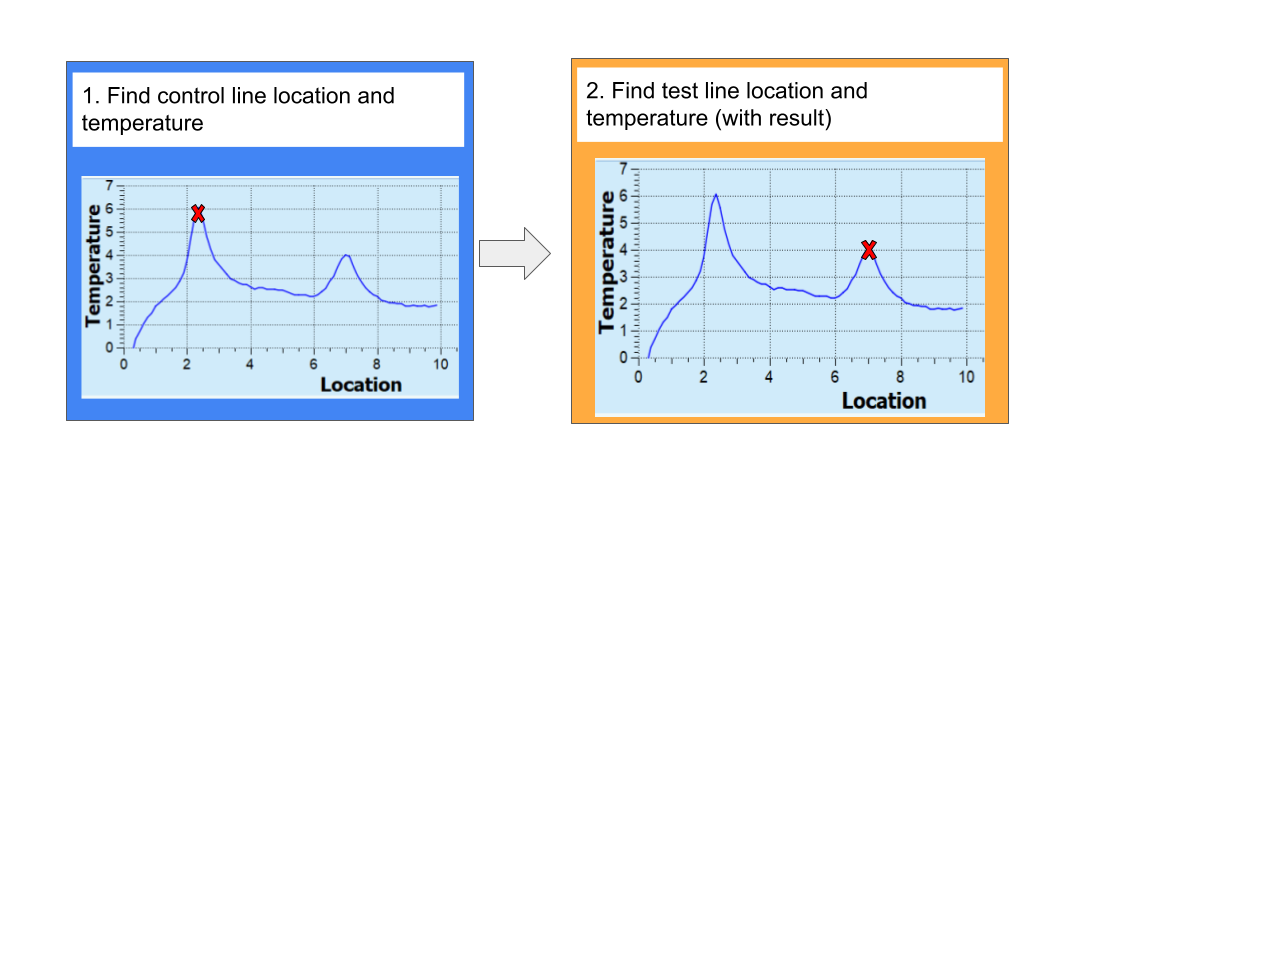
\includegraphics[clip, scale = 0.3]{images/TCA logic a.png}
% \vspace{-5.5cm}
% \label{fig: overarching}
% %\vspace{1.0cm}
% }
% \end{center}
% \caption{Piecewise flowchart of TCA test determination algorithm version 2.0}
% \label{fig: logic}
% \end{figure}

% \newpage

% \begin{figure}[h!] 
% \ContinuedFloat
% \vspace{-1cm}
% %\hspace{0.5cm}
% %\begin{minipage}[b]{\textwidth}

% %\hfill
% \begin{center}
% \subfloat[Detailed process for control line location]{
% 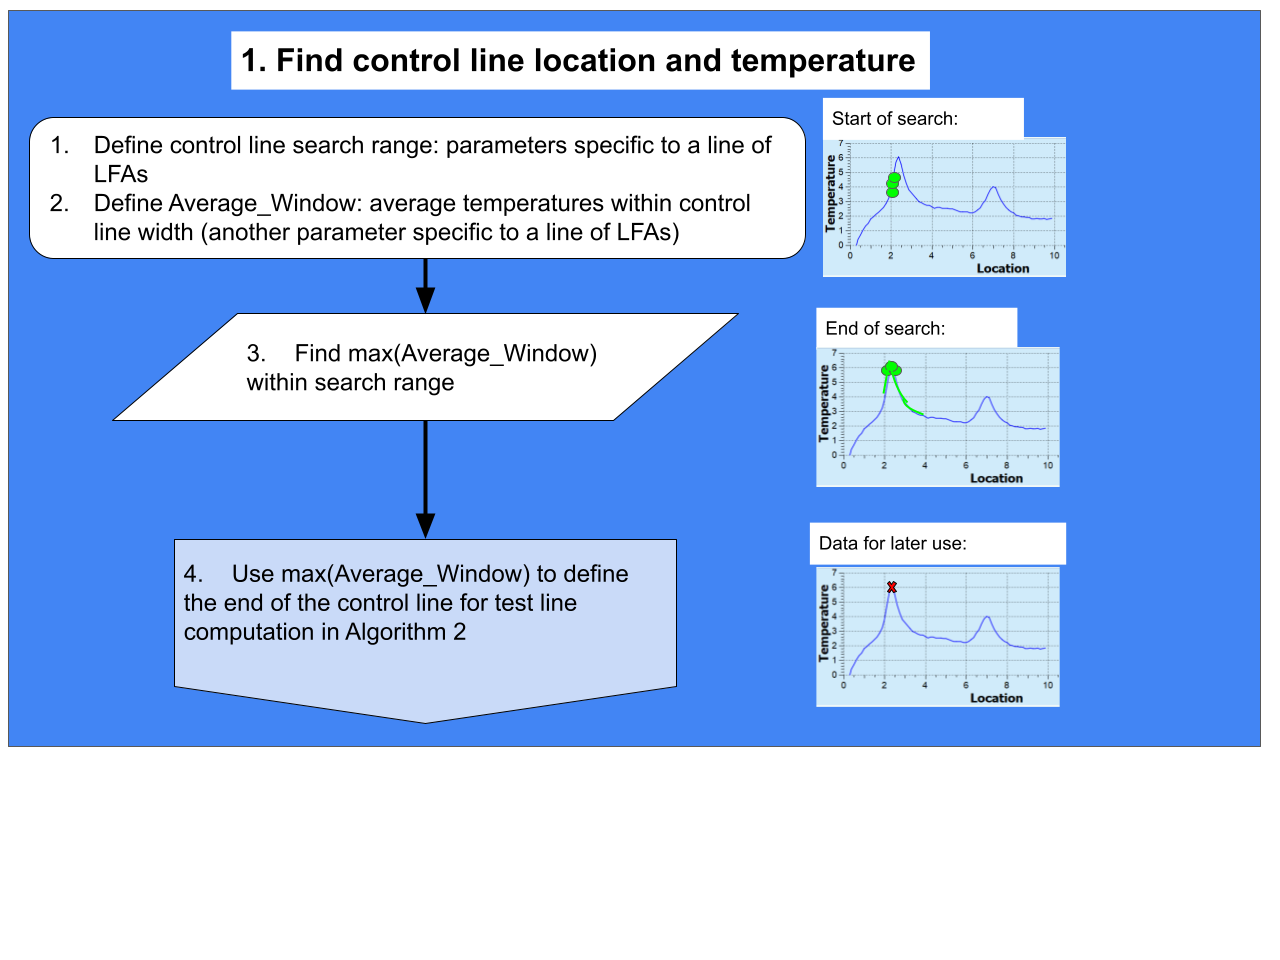
\includegraphics[clip, scale = 0.3]{images/TCA flowchart b.png}
% \vspace{-2cm}
% \label{fig: CL}
% }
% %\end{subfigure}
% %\hspace{10cm}
% \end{center}
% \begin{center}
% \subfloat[Detailed process for final test determination]{
% %\vspace{1cm}
% 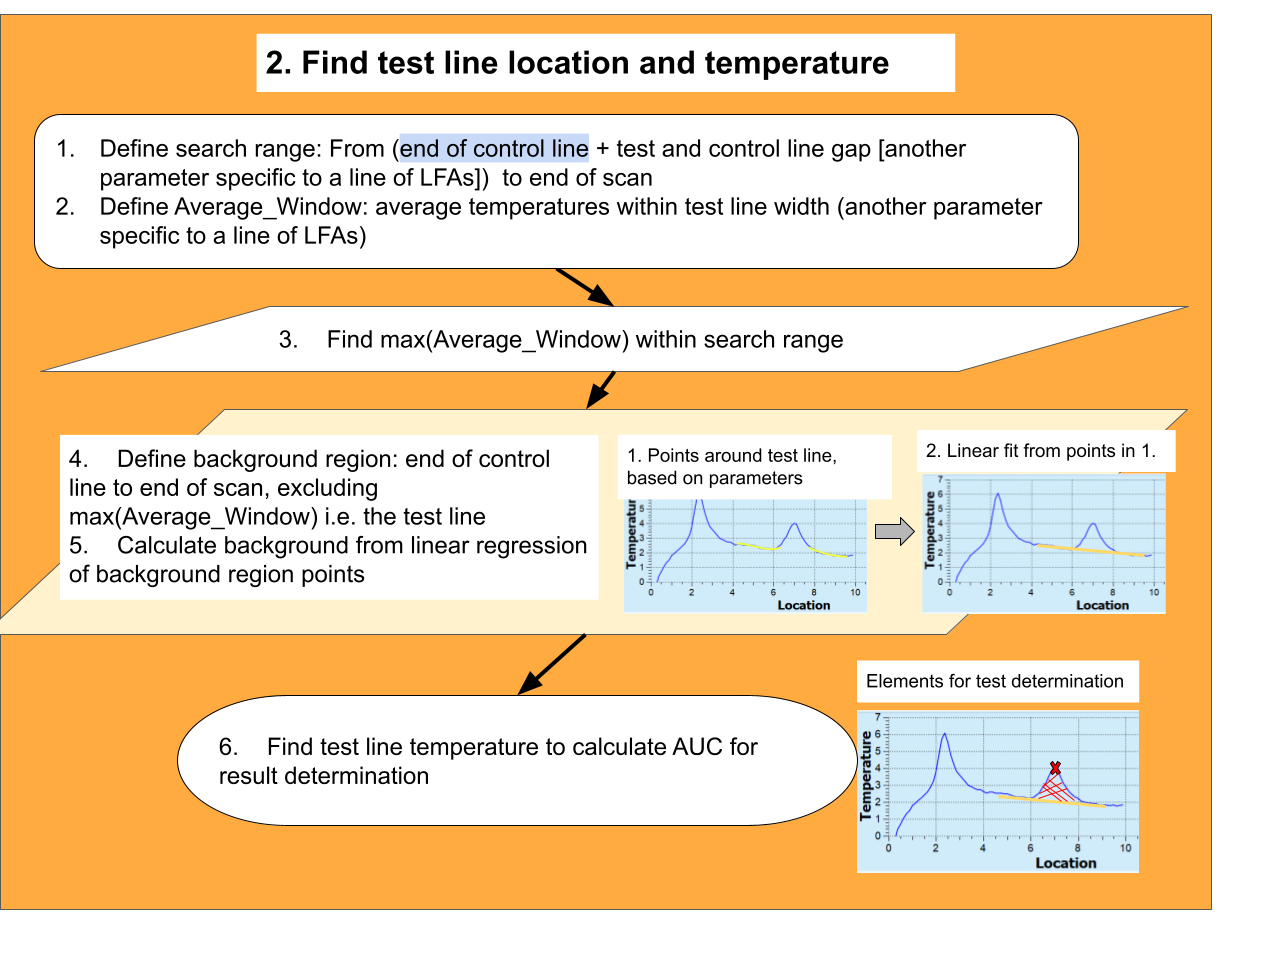
\includegraphics[scale = 0.3]{images/TCA flowchart c.png}
% \label{fig: TL}
% %\vspace{-1cm}
% }
% \vspace{-0.5cm}
% \end{center}
% % \vspace{-1cm}
% \caption{Piecewise flowchart of TCA test determination algorithm version 2.0}
% \hfill
% %\begin{subfigure}[b][3pt][b]{0.2\textwidth}

% \hfill
% \label{fig: logic}
% \vspace{-1cm}
% \end{figure}

% The remainder of my duties involving the TCA reader were validation tests with the 2.0 algorithm and device hardware itself. Before going on to Carnegie Mellon University for graduate school, I trained my replacement and wrote and produced instructional manuals and videos for the reader and GNP synthesis.


\subsection{Aquatic Species Cryopreservation}
Among the many projects of the BHMT group, I was also involved with the cryopreservation of zebrafish embryos. Building off of previous successes of whole zebrafish embryo cryopreservation in the group \cite{Khosla}, we sought to improve primordial germ cell (PGC) cryopreservation with the procedures used in previous work. PGC cryopreservation allows for a simpler target for vitrification and can easily be transplanted in other fish for efficient husbandry \cite{higaki}-- equivalent to cryopreserving whole embryos if not potentially moreso. \\

Once I was proficient in microinjection, a key consideration was removing the yolk from the embryo which I had built using parts already available in the research space (Figure \ref{fig: microyolk}). Difficulties in producing a GFP-plasmid for PGC tagging with collaborators kept this project on indeterminate hold and my results with the yolk extractor were purely preliminary before I had to move on. I believe the core parts were adaptable and did not require the exceptional handling required in the previous work's supplemental video \cite{higaki} with fine-tuning primarily for the long-tipped (LT) pipette.
%%% old figure:
% \newpage
% \vspace{4cm}
% \begin{figure}[h]
% \begin{center}
% \hspace{10cm}
% \fcapside
% \captionsetup[capbesidefigure]
%{justification=raggedright}%
% \thisfloatsetup{capbesideposition=right}
% [\FBwidth]
% [t]
% {\caption{Diagram for building a zebrafish yolk extractor from available magnetic microinjection setup.\label{fig: microyolk}}}
% {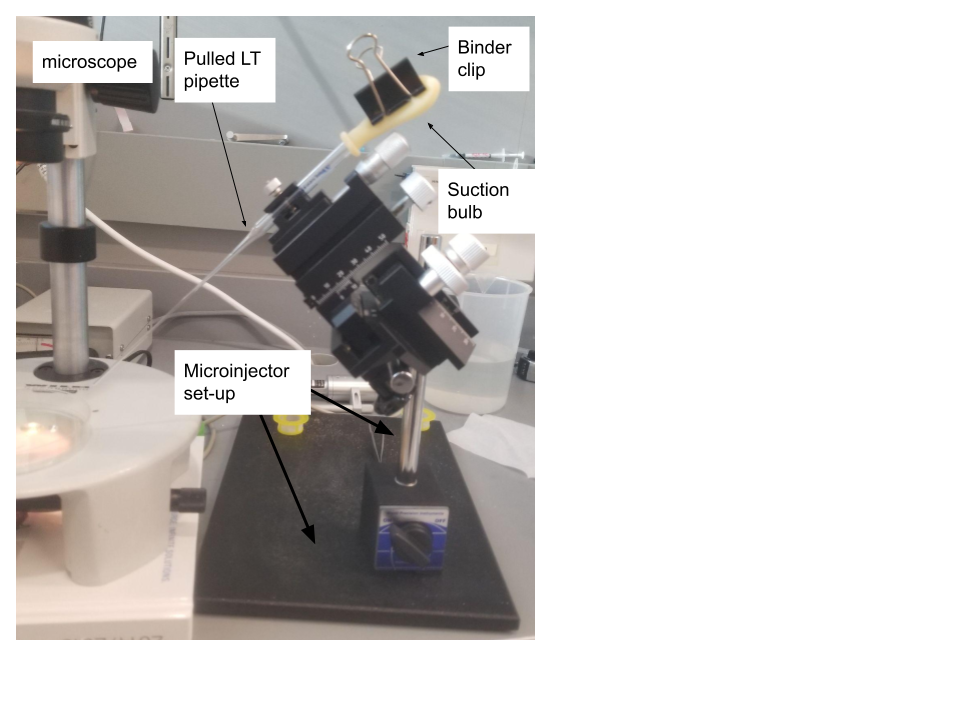
\includegraphics[right, scale = 0.4]{images/Yolk Extraction_embryo digestion.png}}
% \end{center}
% \end{figure}
% \vspace{4cm}
%%% end[old figure]

\begin{SCfigure}[50][h]
\vspace{-1cm}
    % \begin{center}
    % \justifying{
    \hspace{2cm}
    \vspace{5cm}
    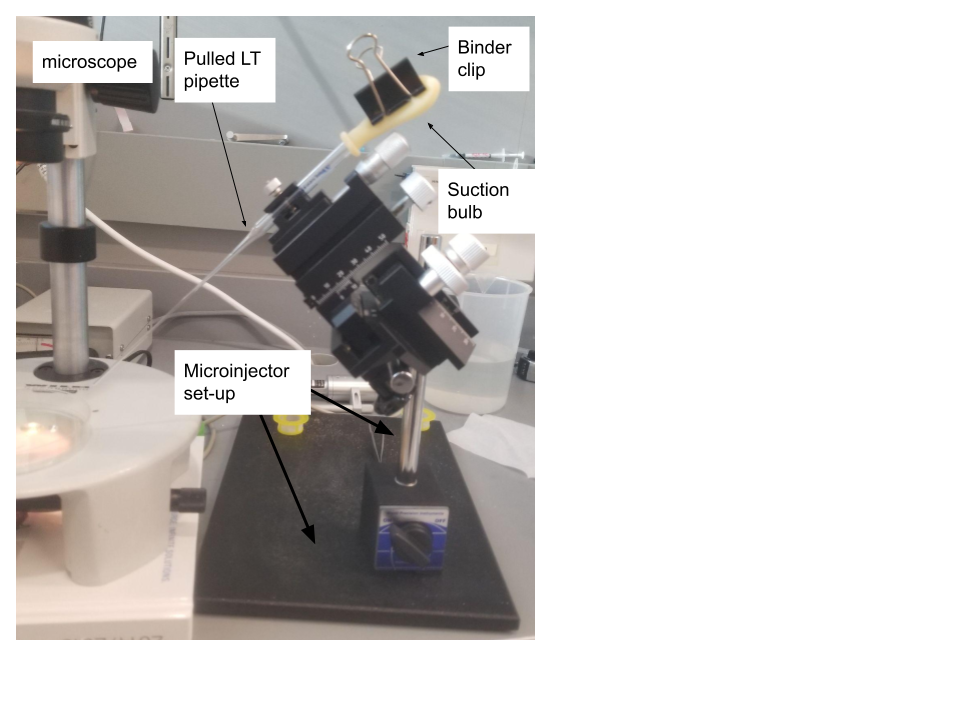
\includegraphics[trim={0 0 16cm 0}, clip, scale = 0.4]{images/Yolk Extraction_embryo digestion.png}    
        \vspace{-5cm}
    % \hspace{-8cm}
    \caption{Diagram for building a zebrafish yolk extractor from available magnetic microinjection setup.}
\label{fig: microyolk}
    % \end{center}
    % \vspace{5cm}
\end{SCfigure}
\newpage
\section{Undergraduate projects at Washington University in St. Louis}
\subsection{WashU Summer Research Fellowship: “Optimization of a nicotine ELISA protocol for use in a vaccine for nicotine addiction”}
My final research project at Washington University in St. Louis (WashU) was with Dr. Jai Rudra where I independently developed an ELISA calibration curve for use in experiments designing a vaccine for drug addiction. Part of this research included a poster presentation where I worked to find the points for a calibration curve of control anti-nicotine antibodies(Figure \ref{fig: ELISA}). This project served as my introduction to a wet-lab environment and was where I learned the importance of plate-based assays for broader projects.

During the year I was with Dr. Rudra, I received an institutional summer research fellowship as well as presented my research at the WashU Undergraduate Fall Research Symposium. I also began work to conjugate nicotine and BSA(bovine serum albumin) with an EDC crosslinker. However, during March 2020 I had to put all projects on indefinite hold during campus lockdown. 
%\begin{wrapfigure}{r} {0.4\textheight}
\begin{figure}[h]
\centering
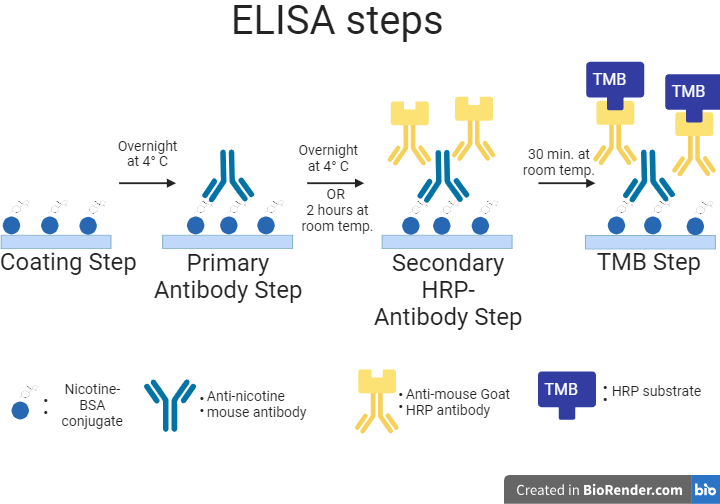
\includegraphics[scale=0.4]{images/19 Poster ELISA diagram copy.png}
\caption{Overview of ELISA protocol I optimized for nicotine and anti-nicotine mouse antibodies. Made in Biorender.}
\label{fig: ELISA}
\end{figure}
\newpage
%\end{wrapfigure}

\subsection{\textit{Biomaterials Science} Draft-RO1 Group Final Project: "Playing with our Food: Advancements in Artificial Meat"}
This class introduced me to polymer chemistry and its importance in a biomedical context beginning with surface chemistry as well as applications. The final project in this class was a mock-RO1 grant and presentation with teams of four. Since my group did not come from similar research backgrounds, I suggested we do a project on something novel like artificial meat so we could cover a wide range of research and because we all were also some combination of foodie or cook.

Our idea for the final project was that artificial meat at the time needed characterization and complex patterning to be a convincing substitute for a complex cut like steak. Characterization consisted of two fronts: (1) a lack of data on viscoelastic properties for steak, but also substitutes of varying similarity: ground beef, tofu, and meat substitute products (2) a lack of understanding of what the human mouth could discern and detect in terms of both taste and texture.  3D printing would then be used to precisely deposit striations or fibers that would mimic real meat's complex mixture of tissue (Figure \ref{fig: steak comparison}).
% \begin{figure}[h!]
\begin{figure}[h]
% \begin{wrapfigure}[h]
\centering
\begin{subfigure}[t]{0.2\textwidth}
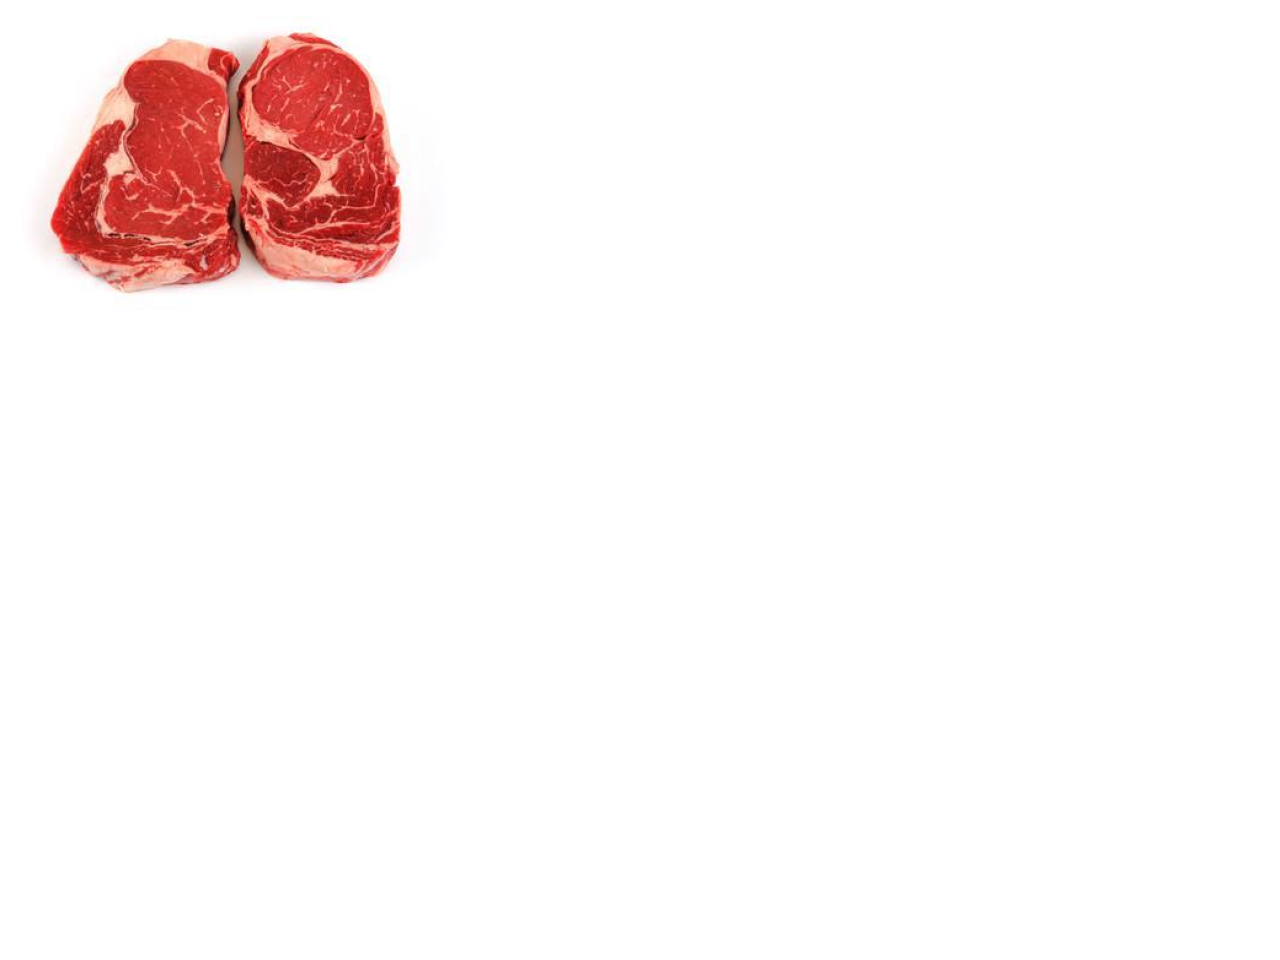
\includegraphics[trim={2cm 0 5cm 0},clip,scale=0.3]{images/actual stock steak a.png}
\vspace{-7cm}
\caption{Reference stock image of a ribeye steak}
\label{fig: steak}
\end{subfigure}
\hspace{1cm}
\begin{subfigure}[t]{0.2\textwidth}

\includegraphics[trim={3cm 0 5cm 0}, clip,scale=0.3]{images/biorendered steak b.png}
\vspace{-7cm}
\caption{Simple striation, only a c-shaped pattern of fat striation}
\label{fig: just c}
\end{subfigure}
\hspace{1cm}
\begin{subfigure}[t]{0.2\textwidth}
% \vspace{-5cm}

\includegraphics[trim={3cm 0 0 0}, clip,scale=0.3]{images/biorendered steak c.png}
\vspace{-7cm}
\caption{ \noindent\hspace*{-2.8mm} Incorporating random spotting with Figure \ref{fig: just c} to better mimic Figure \ref{fig: steak}}
\label{fig: c_rand}
\end{subfigure}
\vspace{-4cm}
\caption{Comparison of actual steak (a) to extremely simplified substitute (b) with closest proposed imitation(c)}
\label{fig: steak comparison}
\end{figure}

\subsection{\textit{Biomacromolecules Design and Engineering} PyMol tutorial: Sculpting, Filtering, and Density Wizards}
This class introduced me to PyMOL, a molecular visualization tool, and the RCSB Protein Data Bank. With these tools, I could better grasp the biochemical concepts behind protein functions and interactions. As part of the course I presented on how to use the PyMOL's density map tool. This tool allows one to visualize and highlight electron densities of the desired protein and/or its surroundings (Figure \ref{fig: pym dens}).
% The sculpting tool allows the user to make conformation changes and then observe the change in properties such as steric hindrance.
\begin{figure}
\begin{center}
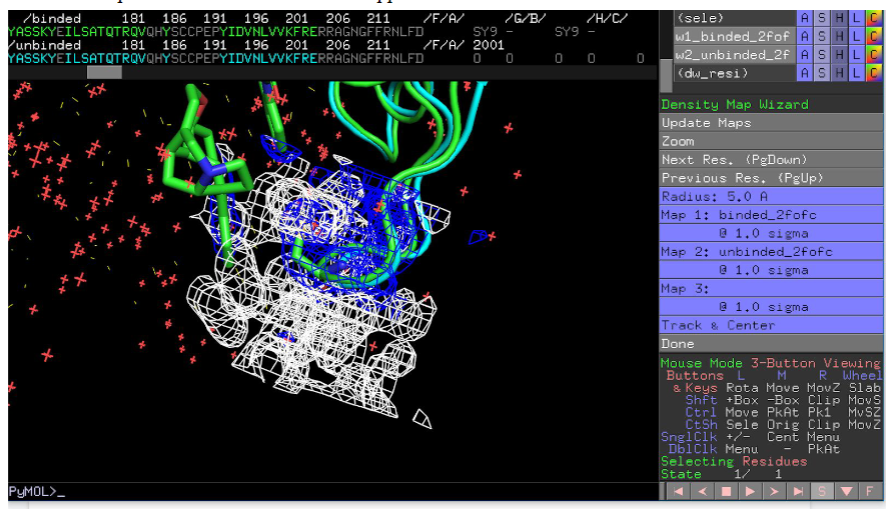
\includegraphics[scale=0.7]{images/sculpting wizard tutorial.png}
\caption{Screenshot taken from PyMOL electron density map tutorial. Here, strychnine's bound and unbound forms are being compared. }
\label{fig: pym dens}
\end{center}
\end{figure}
% \end{wrapfigure}
\newpage
\printbibliography[heading = bibintoc]
\newpage
% \import{resume}
\addcontentsline{toc}{section}{Resume}
% \documentclass[class=article, crop=false]{standalone}
%-------------------------
% Resume in Latex
% Author
% License : MIT
%------------------------
% NOTE: * needed to exclude sections from ToC

%---- Required Packages and Functions ----
% \usepackage{latexsym}
% \usepackage{xcolor}
% \usepackage{float}
% \usepackage{ragged2e}
% \usepackage[empty]{fullpage}
% \usepackage{wrapfig}
% \usepackage{lipsum}
% \usepackage{tabularx}
% \usepackage{titlesec}
% \usepackage{geometry}
% \usepackage{marvosym}
% \usepackage{verbatim}
% \usepackage{enumitem}
% \usepackage[hidelinks]{hyperref}
% \usepackage{fancyhdr}
% \usepackage{fontawesome5}
% \usepackage{multicol}
% \usepackage{graphicx}
% \usepackage{cfr-lm}
% \usepackage[T1]{fontenc}
% \usepackage{fontspec}
% \setlength{\multicolsep}{0pt} 
% \pagestyle{fancy}
% \fancyhf{} % clear all header and footer fields
% \fancyfoot{}
% \renewcommand{\headrulewidth}{0pt}
% \renewcommand{\footrulewidth}{0pt}
% \geometry{left=0.5 in, top=0.5 in, right=0.5 in, bottom=0.5 in}
% Adjust margins
%\addtolength{\oddsidemargin}{-0.5in}
%\addtolength{\evensidemargin}{-0.5in}
%\addtolength{\textwidth}{1in}
% \usepackage[most]{tcolorbox}
\tcbset{
	frame code={}
	center title,
	left=0pt,
	right=0pt,
	top=0pt,
	bottom=0pt,
	colback=gray!20,
	colframe=white,
	width=\dimexpr\textwidth\relax,
	enlarge left by=-2mm,
	boxsep=4pt,
	arc=0pt,outer arc=0pt,
}
% \hypersetup{
%     colorlinks=true,
%     linkcolor=cyan,
%     filecolor=magenta,      
%     urlcolor=blue
%     }

\urlstyle{same}

\raggedright
\setlength{\tabcolsep}{0in}

% Sections formatting
\titleformat{\section}{
  \vspace{-4pt}\scshape\raggedright\large
}{}{0em}{}[\color{black}\titlerule \vspace{-7pt}]

%-------------------------
% Custom commands
\newcommand{\resumeItem}[2]{
  \item{
    \textbf{#1}{\hspace{0.5mm}#2 \vspace{-0.5mm}}
  }
}

\newcommand{\resumePOR}[3]{
\vspace{0.5mm}\item
    \begin{tabular*}{0.97\textwidth}[t]{l@{\extracolsep{\fill}}r}
        \textbf{#1}\hspace{0.3mm}#2 & \textit{\small{#3}} 
    \end{tabular*}
    \vspace{-2mm}
}

\newcommand{\resumeSubheading}[4]{
\vspace{0.5mm}\item[]
    \begin{tabular*}{0.98\textwidth}[t]{l@{\extracolsep{\fill}}r}
        \textbf{#1} & {\footnotesize{#4}} \\
        {\footnotesize{#3}} &  \footnotesize{#2}\\
    \end{tabular*}
    \vspace{-2.4mm}
}

\newcommand{\resumeJob}[5]{
% \vspace{0.5mm}
\item[]
    \begin{tabular*}{0.98\textwidth}[t]{l@{\extracolsep{\fill}}r}
        \textbf{#1} & {\footnotesize{#2}} \\
        \footnotesize{{#3}} & \footnotesize{#4}\\
        \textbf{#5}
    \end{tabular*}
    \vspace{-2.4mm}
}
\newcommand{\subproject}[1]{
\vspace{-2mm}\item[] \textbf{#1}\vspace{-2mm}
    
}

\newcommand{\resumeSubItem}[2]{\resumeItem{#1}{#2}\vspace{-4pt}}

\renewcommand{\labelitemii}{$\bullet$}
% \renewcommand{\labelitemiii}{$\circ$}
%\renewcommand{\labelitemi}{$\vcenter{\hbox{\tiny$\bullet$}}$}

\newcommand{\resumeSubHeadingListStart}{\begin{itemize}[leftmargin=*,labelsep=0mm]}
\newcommand{\resumeHeadingSkillStart}{\begin{itemize}[leftmargin=*,itemsep=1.7mm, rightmargin=2ex]}
\newcommand{\resumeItemListStart}{\begin{justify}\begin{itemize}[leftmargin=3ex, rightmargin=2ex, noitemsep,labelsep=1.2mm,itemsep=0mm]\small}

% \newcommand{\resumeSubHeadingListEnd}{\end{itemize}\vspace{2mm}}
\newcommand{\resumeSubHeadingListEnd}{\end{itemize}\vspace{-2mm}}
\newcommand{\resumeHeadingSkillEnd}{\end{itemize}\vspace{-2mm}}
\newcommand{\resumeItemListEnd}{\end{itemize}\end{justify}\vspace{-2mm}}
% \newcommand{\cvsection}[1]{%
% \vspace{2mm}
% \begin{tcolorbox}
%     \textbf{\large #1}
% \end{tcolorbox}
%     \vspace{-4mm}
% }

\newcolumntype{L}{>{\raggedright\arraybackslash}X}%
\newcolumntype{R}{>{\raggedleft\arraybackslash}X}%
\newcolumntype{C}{>{\centering\arraybackslash}X}%
%---- End of Packages and Functions ------

%-------------------------------------------
%%%%%%  CV STARTS HERE  %%%%%%%%%%%
%%%%%% DEFINE ELEMENTS HERE %%%%%%%
\newcommand{\name}{Jesse Shen} % Your Name
%\newcommand{\course}{Your Program} % Your Program
%\newcommand{\roll}{xxxxxxx} % Your Roll No.
\newcommand{\phone}{503-956-0562} % Your Phone Number
%emaila used in portfolio

% \begin{document}
\fontfamily{cmr}\selectfont
\setmainfont{Times New Roman}
%----------HEADING-----------------

\begin{center}
			{\Large \scshape {\Large \name}}\\ 
			\href{mailto:\emaila}{\raisebox{0.0\height}{\footnotesize \faEnvelope}\ {\emaila}} \
            % \smallskip {{\footnotesize \faPhone}\ \phone} \ \smallskip
			% \href{https://www.linkedin.com/in/jesse-shen-78abba175/}{\footnotesize \faLinkedin}\ \smallskip
		 \href{https://github.com/jesse12shen}{\raisebox{0.0\height}{\footnotesize \faGithub}\ {Jesse12Shen}}\\
         % {Mountain View, CA}
   % \textbf{Summary:} 
   % I am a biomedical engineer with an academic background seeking positions at the intersection between AI and healthcare. 
\end{center}

%\parbox{2.35cm}{%
%\includegraphics[width=2.35cm,clip]{Mnit_logo_bw.png}}
% \parbox{\dimexpr\linewidth-2.8cm\relax}{
% \begin{tabularx}{\linewidth}{L r} \\
%   \textbf{\Large \name} & {\raisebox{0.0\height}{\footnotesize \faPhone}\ \phone}\\
%   \href{mailto:\emaila}{\raisebox{0.0\height}{\footnotesize \faEnvelope}\ {\emaila}} &
%   \href{https://www.linkedin.com/in/jesse-shen-78abba175/}{\raisebox{0.0\height}{\footnotesize \faLinkedin}\ }
  %\href{mailto:\emailb}{\raisebox{0.0\height}{\footnotesize \faEnvelope}\ {\emailb}}\\
  %{Your Course} &  \href{https://yourGithubProfile.com/}{\raisebox{0.0\height}{\footnotesize \faGithub}\ {GitHub Profile}} \\
  %{Malaviya National Institute Of Technology, Jaipur} & \href{https://www.yourLinkedinProfile.com/in/}{\raisebox{0.0\height}{\footnotesize \faLinkedin}\ {LinkedIn Profile}}
% \end{tabularx}
% }
% \parbox{3.0cm}{%
% \flushright \includegraphics[width=2cm,clip]{nitp_logo.png}
% }

%-----------EDUCATION-----------

    
    \section*{\textbf{Experience}}
\resumeSubHeadingListStart
    \resumeJob {Intuit}{2026}{Contract Software Engineer}{Mountain View, CA}{Fintech Event Bus Migration Effort}
     \resumeItemListStart
    \item {Migrated tens of applications to new Kafka topic clusters using a 7-step workflow, maintaining near-zero downtime across distributed fintech systems.}
    \item {Designed and evaluated an AI agent to automate portions of workflow and increase developer throughput by 120\%}
    \item {This AI agent, after team contributions, employed up to 9 MCPs to access API's and data across Intuit with varying configurations and development status, and improved developer throughput by 150\%}
    \item {Tools \& technologies used: Kafka, Spark, Beam, Maven, Kubernetes, AWS, Docker, Linux, Claude Code, Numaflow, Java, Python}
    \resumeItemListEnd
    \resumeJob {Revature}{2025}{Java Intern}{Remote}{Spring Social media blog API}
      \resumeItemListStart
      \item \textcolor{blue}{{\url{https://github.com/jesse12shen/jesse12shen-pep-spring-project}}} 
    \item{Implemented all user stories, i.e. requested features using Spring Boot and an MVC design pattern}
    \item {Tools \& technologies used: Spring Boot, SQL, JaCoCo, JUnit, REST APIs, Agile methodology}
    % \vspace{-2 mm}
    \resumeItemListEnd

        % \item{Ran flow cytometry to characterize clonogenic thymic epithelial cells adhered to feeder cells}

    % \vspace{1.0mm}
      % \vspace{-2.0mm}


    % \item{Performed antibody conjugation for use in lab-based lateral flow assays involving  UV-VIS, DLS, and PAGE.}
    % \item{Reduced MATLAB computation time by 50\% through modular refactoring}
    % \item{Assembled lateral flow assays with lateral flow reagent dispenser.}
    % \resumeItemListStart
    \resumeJob {Carnegie Mellon University Department of Biomedical Engineering}{2022 - 2023}{Graduate Student Researcher}{Pittsburgh, PA}
      {Thymus-on-a-chip}
  % {Extracellular Vesicle (EV)-based Cancer Diagnostics}
  \resumeItemListStart
  %     \item {Led integration of next-generation sequencing into a cancer methylation diagnostic workflow, using ddPCR and qPCR to validate signal across a multi-modal genomics pipeline}\\
  %     \resumeItemListEnd
  %     \vspace{-4.0mm}
  % \subproject{Thymus-on-a-chip}
  %     \vspace{-2.0mm}
      % \resumeItemListStart
    % \item {Developed PDMS organ-on-a-chip design as part of an in vitro microfluidic thymus device in a collaborative project with immunologists.}
    \item{Designed organ-on-a-chip device in collaboration with immunologists, gaining direct experience translating between engineering constraints and domain-expert scientific requirements}
    \resumeItemListEnd
        \resumeJob
      {University of Minnesota- Department of Mechanical Engineering}{2020 - 2022}{Research Technician}{Minneapolis, MN}{Thermal contrast amplification for use in lateral flow assays / VigilantDx Startup}
      %\vspace{-2.0mm}
      \resumeItemListStart
     \item{Performed quantitative signal detection and noise characterization across sample runs to establish femtomolar detection thresholds for COVID antigen assay.}
    \item{Developed and proposed antibody conjugation verification assay, independently scoping and validating a novel measurement methodology}
    % \item {Performed validation tests for prototype diagnostic medical device.}
    \item {Served as lead author in VigilantDx LFA reader v1.0.16 user manual and produced promotional material including shareholder videos.}
    \item{Published in ACS Applied Nano Materials, 2021}
        \resumeItemListEnd
    \resumeSubHeadingListEnd

\vspace{-5.5mm}
\section*{\textbf{Projects}}
% \resumeSubHeadingListStart
    % \resumeItemListStart
    % \resumeJob {Revature Bootcamp Capstone Project}{January 2025 - Present}{\textbf{Spring Social media blog API}}{}{{\normalfont\textcolor{blue}{\url{https://github.com/jesse12shen/jesse12shen-pep-spring-project}}}}
    
    % \item{Tools \& technologies used: Spring Boot, Spring Data, Spring Framework, Java, Javalin, JDBC, SQL, RESTful APIs, Agile Scrum}
    % \item {A social media application with an api backend without a frontend. Can manage user accounts and messages that they submit to the application, users will be able to see all of the messages posted to the site as well as the messages posted by a particular user, as well as process actions like logins, registrations, message creations, message updates, and message deletions.}
    % \item{Implemented all user stories, i.e. requested features using Spring Boot and an MVC design pattern}
    %     \resumeItemListEnd
% \vspace{-2.0mm}
    \resumeItemListStart
        \resumeJob
          {Carnegie Mellon University: \textit{Introduction to Deep Learning 11-785}}{2024}{{\normalfont\textcolor{blue}{{\url{https://github.com/rohanchawla23/11785Project}}}}}{}{}
                \vspace{-2.0mm}
      % \resumeItemListStart
      \item {Compared a selective structured state space model(Mamba) to a transformer baseline for cancer diagnostics with EHR/ICD-10-CM data as part of a 4-person team. I ran the baseline control locally and wrote the literature review.}
      % \item{Implemented a Transformer using patient EHR, ICD-10-CM data}
      % \item{Wrote a proposal for a transformer model for early cancer detection based on previous literature.}
      \item{Conducted literature review on prior AI cancer diagnostic approaches to inform architecture decisions and situate results within the broader research landscape}
      \item{Performed ablation studies on CNNs and LSTMs using remote GCP/AWS Linux instances, developing intuition for model tradeoffs relevant to clinical data}
    \item{Tools \& technologies used: Pytorch, WandB, Kaggle, NLP, GCP, AWS, OpenAI, Pandas, matplotlib, Jupyter, Python}
      \vspace{-2 mm}
      \resumeItemListEnd
    \resumeItemListStart
    \resumeJob{Restaurant Tag Search}{2023}{\normalfont\textcolor{blue}{\url{https://github.com/jesse12shen/Restaurant_tag_search.git}}}{}{}
      % {} %Project Name, Location Name
       %Event Dates
       \vspace{-2 mm}
        \item {I wanted to look at clustering restaurant reviews based on mentions of certain words after working on a logistic regression involving restaurant reviews.}
        \item {Tools \& technologies used: Python, Pandas, NLP (GLoVE embedding)}
    \resumeItemListEnd
    % \resumeSubHeadingListEnd
    %     \resumeItemListStart
    % \resumeJob{Restaurant Tag Search}{2023}{Based off \textit{Introduction to Machine Learning} assignment}{ }{\normalfont\textcolor{blue}{\url{https://github.com/jesse12shen/Restaurant_tag_search.git}}}

    % \section{\textbf{Other Experience}}
        % \resumeItemListStart
      
\section*{\textbf{Education}}
  \resumeSubHeadingListStart
    \resumeSubheading
      {Carnegie Mellon University}{GPA: 3.63/4.00}
      {Master of Science in Biomedical Engineering}{2024}
                   % \item{\textbf{Relevant Coursework}\footnotesize{: Introduction to Deep Learning, Introduction to Machine Learning, Neural Computation, Immunology, Medical Device Innovation and Realization, Biomaterial Host Interactions in Regenerative Medicine, Advanced Physiology}}
    \resumeSubheading
      {Washington University in St. Louis }{GPA: 3.65/4.00}
      {Bachelor of Science in Biomedical Engineering}{2020}
             % \item{\textbf{Relevant Coursework}\footnotesize{: Biomaterials Science, Biomacromolecule Engineering, Quantitative Physiology,  Molecular and Cellular Engineering, Organic Chemistry}}
  \resumeSubHeadingListEnd

% \vspace{-7mm}
%

                
  % \resumeSubHeadingListStart
  %   \resumeJob
  %         {Carnegie Mellon University: \textit{Medical Device Innovation and Realization}}{January 2023 - May 2023}{Group Technical Lead}{Pittsburgh, PA}{Cell encapsulation for Type-1 diabetes therapy}
                % \vspace{-4.0mm}
  %     \resumeItemListStart
  %     \item{Used Solidworks to design a 3D printed model of our cell encapsulation device involving Cura and FDM}
  %     \item{Performed diffusion simulations in COMSOL}
  %     \resumeItemListEnd
  %   \resumeSubHeadingListEnd
      % \vspace{-2.0mm}


    % \resumeSubHeadingListEnd
    
    % \resumeItemListStart
    % \resumeJob{Restaurant Tag Search}{2023}{Based off \textit{Introduction to Machine Learning} assignment}{ }{\normalfont\textcolor{blue}{\url{https://github.com/jesse12shen/Restaurant_tag_search.git}}}
    %   % {} %Project Name, Location Name
    %    %Event Dates
      
    %     \item {Tools \& technologies used: Python, Pandas, NLP (GLoVE embedding)}
    %     \item {I wanted to look at clustering restaurant reviews based on mentions of certain words after working on a logistic regression involving restaurant reviews. Worked around academic policy by pre-training model and only uploading weights, but code is available upon request.}
    % \resumeItemListEnd
    % \vspace{-4mm}
\vspace{-3mm}


%-----------Technical skills-----------------
\section*{\textbf{Technical Skills}}
 \begin{itemize}[leftmargin=0.05in, label={}]
    \small{
 %    \textbf{Languages}{: Chinese(intermediate } \\
 %    \textbf{Developer Tools}{: } \\
 \item{\textbf{Libraries}{: Pytorch $\cdot$ Git $\cdot$ GCP $\cdot$ AWS $\cdot$ Kafka $\cdot$ Spark $\cdot$ Beam $\cdot$ Maven $\cdot$ Kubernetes $\cdot$ Claude Code $\cdot$ Pandas $\cdot$ matplotlib $\cdot$ Numaflow}}
 \item{ \textbf{Languages}: MATLAB $\cdot$ Python $\cdot$ Java $\cdot$ R $\cdot$ SQL $\cdot$ GoLang $\cdot$ JavaScript }
 \item{\textbf{Misc. Skills} : device development $\cdot$ data visualization $\cdot$ SOP writing}
    }
 \end{itemize}
 \vspace{-16pt}
% \end{document}

% 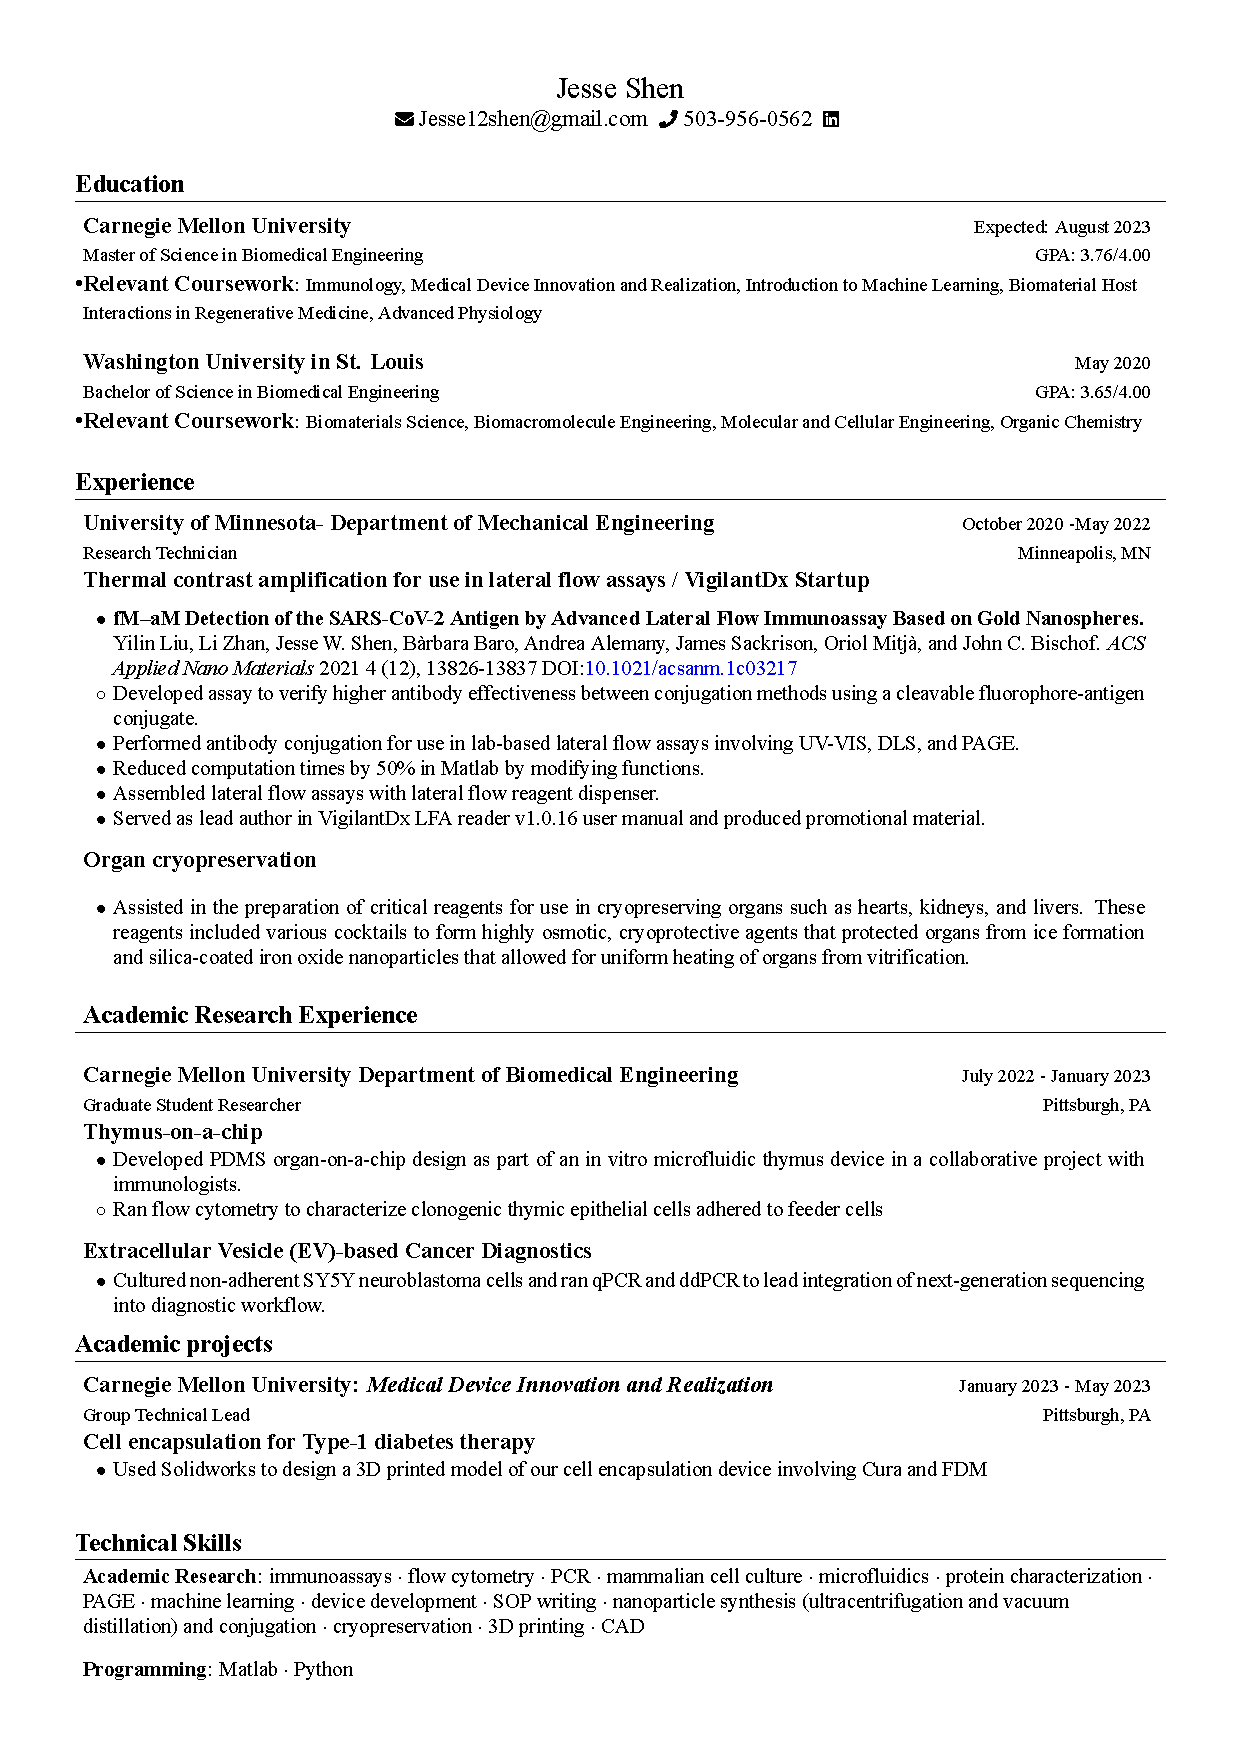
\includepdf[pages=-]{23_Resume_Jesse_modified_3d_print (4).pdf}
\end{document}